\documentclass[a4paper,11pt]{article}\usepackage[]{graphicx}\usepackage[]{color}
%% maxwidth is the original width if it is less than linewidth
%% otherwise use linewidth (to make sure the graphics do not exceed the margin)
\makeatletter
\def\maxwidth{ %
  \ifdim\Gin@nat@width>\linewidth
    \linewidth
  \else
    \Gin@nat@width
  \fi
}
\makeatother

\definecolor{fgcolor}{rgb}{0.345, 0.345, 0.345}
\newcommand{\hlnum}[1]{\textcolor[rgb]{0.686,0.059,0.569}{#1}}%
\newcommand{\hlstr}[1]{\textcolor[rgb]{0.192,0.494,0.8}{#1}}%
\newcommand{\hlcom}[1]{\textcolor[rgb]{0.678,0.584,0.686}{\textit{#1}}}%
\newcommand{\hlopt}[1]{\textcolor[rgb]{0,0,0}{#1}}%
\newcommand{\hlstd}[1]{\textcolor[rgb]{0.345,0.345,0.345}{#1}}%
\newcommand{\hlkwa}[1]{\textcolor[rgb]{0.161,0.373,0.58}{\textbf{#1}}}%
\newcommand{\hlkwb}[1]{\textcolor[rgb]{0.69,0.353,0.396}{#1}}%
\newcommand{\hlkwc}[1]{\textcolor[rgb]{0.333,0.667,0.333}{#1}}%
\newcommand{\hlkwd}[1]{\textcolor[rgb]{0.737,0.353,0.396}{\textbf{#1}}}%

\usepackage{framed}
\makeatletter
\newenvironment{kframe}{%
 \def\at@end@of@kframe{}%
 \ifinner\ifhmode%
  \def\at@end@of@kframe{\end{minipage}}%
  \begin{minipage}{\columnwidth}%
 \fi\fi%
 \def\FrameCommand##1{\hskip\@totalleftmargin \hskip-\fboxsep
 \colorbox{shadecolor}{##1}\hskip-\fboxsep
     % There is no \\@totalrightmargin, so:
     \hskip-\linewidth \hskip-\@totalleftmargin \hskip\columnwidth}%
 \MakeFramed {\advance\hsize-\width
   \@totalleftmargin\z@ \linewidth\hsize
   \@setminipage}}%
 {\par\unskip\endMakeFramed%
 \at@end@of@kframe}
\makeatother

\definecolor{shadecolor}{rgb}{.97, .97, .97}
\definecolor{messagecolor}{rgb}{0, 0, 0}
\definecolor{warningcolor}{rgb}{1, 0, 1}
\definecolor{errorcolor}{rgb}{1, 0, 0}
\newenvironment{knitrout}{}{} % an empty environment to be redefined in TeX

\usepackage{alltt}
 
\usepackage{hyperref}
\usepackage{graphicx}
\usepackage{amssymb,amsmath}
\usepackage{bm}
\usepackage[margin=1in]{geometry}
\usepackage{color}
\usepackage{setspace}
\usepackage{multirow}
\usepackage{booktabs}
\usepackage{array}
\usepackage[normalem]{ulem}

\newcommand{\zerob} {{\bf 0}}
\newcommand{\oneb} {{\bf 1}}
\newcommand{\expect} {{\mathbb{E}}}
\newcommand{\pt} {\tilde{p}}
\newcommand{\alphat} {\tilde{\alpha}}
\newcommand{\betat} {\tilde{\beta}}
\newcommand{\pb} {\bar{p}}
\newcommand{\thetab} {{\boldsymbol{\theta}}}
\newcommand{\alphab} {{\boldsymbol{\alpha}}}
\newcommand{\kappab} {{\boldsymbol{\kappa}}}
\newcommand{\sigmab} {{\boldsymbol{\sigma}}}
\newcommand{\nub} {{\boldsymbol{\nub}}}
\newcommand{\gammab} {{\boldsymbol{\gamma}}}
\newcommand{\deltab} {{\boldsymbol{\delta}}}
\newcommand{\Deltab} {{\boldsymbol{\Delta}}}
\newcommand{\etab} {{\boldsymbol{\eta}}}
\newcommand{\Thetab} {{\boldsymbol{\Theta}}}
\newcommand{\varthetab} {{\boldsymbol{\vartheta}}}
\newcommand{\Yset} {\mathcal{Y}}
\newcommand{\Xset} {\mathcal{X}}
\newcommand{\intd} {\textrm{d}}
\newcommand{\phib} {\boldsymbol{\phi}}
\newcommand{\zetab} {\boldsymbol{\zeta}}
\newcommand{\psib} {\boldsymbol{\psi}}
\newcommand{\Sigmawinv} {{\boldsymbol{\it \Sigma}}_w^{-1}}
\newcommand{\Sigmamat} {{\bm \Sigma}}
\newcommand{\Sigmamatt} {\widetilde{\boldsymbol{\Sigma}}}
\newcommand{\Qmatt} {\widetilde{\textbf{Q}}}
\newcommand{\muvect} {\widetilde{\boldsymbol{\mu}}}
\newcommand{\Psib} {{\bm \Psi}}
\newcommand{\Upsilonmat} {{\boldsymbol{\it \Upsilon}}}
\newcommand{\Lambdamat} {\mathbf{\Lambda}}
\newcommand{\Gammamat} {{\boldsymbol{\it \Gamma}}}
\renewcommand{\Gammamat} {{\boldsymbol{\Gamma}}}
\newcommand{\Pimat} {{\boldsymbol{\it \Pi}}}
\newcommand{\Amat} {\textbf{A}}
\newcommand{\Bmat} {\textbf{B}}
\newcommand{\Dmat} {\textbf{D}}
\newcommand{\Gmat} {\textbf{G}}
\newcommand{\Lmat} {\textbf{L}}
\newcommand{\Qmat} {\textbf{Q}}
\newcommand{\Rmat} {\textbf{R}}
\newcommand{\Tmat} {\textbf{T}}
\newcommand{\Qt} {\widetilde{\textbf{Q}}}
\newcommand{\Qtinv} {\widetilde{\textbf{Q}}^{-1}}
\newcommand{\Mmat} {\textbf{M}}
\newcommand{\Cmat} {\mathbf{C}}
\newcommand{\Jmat} {\mathbf{J}}
\newcommand{\cmat} {\textbf{c}}
\newcommand{\Kmat} {\textbf{K}}
\newcommand{\Zmat} {\textbf{Z}}
\newcommand{\Xmat} {\textbf{X}}
\newcommand{\Xvec} {\mathbf{X}}
\newcommand{\Imat} {\textbf{I}}
\newcommand{\Umat} {\textbf{U}}
\newcommand{\Pmat} {\textbf{P}}
\newcommand{\Hmat} {\textbf{H}}
\newcommand{\Vmat} {\textbf{V}}
\newcommand{\bvec} {\textbf{b}}
\newcommand{\dvec} {\textbf{d}}
\newcommand{\avec} {\textbf{a}}
\newcommand{\evec} {\textbf{e}}
\newcommand{\hvec} {\textbf{h}}
\newcommand{\xvec} {\textbf{x}}
\newcommand{\yvec} {\textbf{y}}
\newcommand{\zvec} {\textbf{z}}
\newcommand{\wvec} {\textbf{w}}
\newcommand{\vvec} {\textbf{v}}
\newcommand{\svec} {\textbf{s}}
\newcommand{\uvec} {\textbf{u}}
\newcommand{\gvec} {\textbf{g}}
\newcommand{\fvec} {\textbf{f}}
\newcommand{\rvec} {\textbf{r}}
\newcommand{\muvec} {\boldsymbol{\mu}}
\newcommand{\Psix} {{\boldsymbol{\it \Psi}}_{\xvec}}
\newcommand{\Phimat} {{\boldsymbol{\it \Phi}}}
\newcommand{\Psitheta} {{\boldsymbol{\it \Psi}}_{\varthetab}}
\newcommand{\Psia} {{\boldsymbol{\it \Psi}}_{A}}
\newcommand{\Psixinv} {{\boldsymbol{\it \Psi}}_{\xvec}^{-1}}
\newcommand{\vvm} {\boldsymbol {\mathcal \upsilon}}
\newcommand{\upsilonb} {\boldsymbol {\upsilon}}
\newcommand{\betab} {\boldsymbol {\beta}}
\newcommand{\omegab} {\boldsymbol {\omega}}
\newcommand{\Aop}{\boldsymbol{\mathcal{A}}}
\newcommand{\ICE} {\textit{ICE}}
\newcommand{\GIA} {\textit{GIA}}
\newcommand{\GPS} {\textit{GPS}}
\newcommand{\ERS} {\textit{ERS}}
\newcommand{\GR} {\textit{GR}}
\newcommand{\IS} {\textit{IS}}
\newcommand{\ES} {\textit{ES}}
\newcommand{\zeroes}{\mathop{\textrm{zeroes}}}
\newcommand{\odd}{\mathop{\textrm{odd}}}
\newcommand{\even}{\mathop{\textrm{even}}}
\newcommand{\ff} {\textit{ff}}
\newcommand{\fm} {\textit{fm}}
\newcommand{\mf} {\textit{mf}}
\newcommand{\inv} {\textit{inv}}

\renewcommand{\zerob}{\mathbf{0}}
\renewcommand{\v}{\mathbf{v}}
\renewcommand{\u}{\mathbf{u}}
\newcommand{\w}{\mathbf{w}}
\renewcommand{\d}{\mathrm{d}}
\newcommand{\Z}{\mathbf{Z}}
\newcommand{\X}{\mathbf{X}}
\newcommand{\x}{\mathbf{x}}
\newcommand{\Y}{\mathbf{Y}}
\newcommand{\Yvec}{\mathbf{Y}}
\newcommand{\Yt}{\widetilde{\mathbf{Y}}}
\newcommand{\Zvec}{\mathbf{Z}}
%\newcommand{\epsilonb}{\mbox{\boldmath{$\varepsilon$}}}                                                                                                                                                       
\newcommand{\epsilonb}{\boldsymbol{\varepsilon}}
\newcommand{\bS}{\mathbf{S}}
\newcommand{\bK}{\mathbf{K}}
\newcommand{\bI}{\mathbf{I}}
\newcommand{\bR}{\mathbf{R}}
\newcommand{\bC}{\mathbf{C}}
\newcommand{\bB}{\mathbf{B}}
\newcommand{\bP}{\mathbf{P}}
\newcommand{\bQ}{\mathbf{Q}}
\renewcommand{\L}{\mathbf{L}}
\newcommand{\E}{\mathrm{E}}
\newcommand{\cov}{\mathrm{cov}}
\newcommand{\var}{\mathrm{var}}
\newcommand{\Dist}{\mathrm{Dist}}
\renewcommand{\prec}{\mathrm{prec}}
\newcommand{\tr}{\mathrm{tr}}
\newcommand{\diag}{\mathrm{diag}}
\newcommand{\sgn}{\mathrm{sgn}}
\newcommand{\trace}{\mathrm{tr}}
\newcommand{\vect}{\mathrm{vec}}
\newcommand{\Gau}{\mathrm{Gau}}

\newcommand{\RR}{\mathbb{R}}

\newcommand{\s}{\mathbf{s}}
\newcommand{\p}{\mathbf{p}}
\renewcommand{\a}{\mathbf{a}}
\newcommand{\h}{\mathbf{h}}
\renewcommand{\b}{\mathbf{b}}
\renewcommand{\c}{\mathbf{c}}
\newcommand{\z}{\mathbf{z}}


\newcommand{\blambda}{\boldsymbol{\lambda}}
\newcommand{\btheta}{\boldsymbol{\theta}}
\newcommand{\balpha}{\boldsymbol{\alpha}}
\newcommand{\bgamma}{\boldsymbol{\gamma}}
\newcommand{\bbeta}{\boldsymbol{\beta}}
\newcommand{\bzero}{\boldsymbol{0}}
\newcommand{\bmu}{\boldsymbol{\mu}}
\newcommand{\bSigma}{\bm{\Sigma}}




\IfFileExists{upquote.sty}{\usepackage{upquote}}{}
\begin{document}

\begin{abstract}
Here we represent repdoducible code for the simulation study appearing in the paper `Spatio-temporal bivariate statistical models for atmospheric trace-gas inversion', Section 4.1. The code requires the installation of two in-house developed packages for this application, \emph{hmc} and \emph{atminv}. The vignette itself is not `polished', but gives the basic requirements for reproducing the figures and values given in the main text.

\end{abstract}

\section{Setup}

To run the simulation study, you need to first install the packages `atminv' and `hmc'. You can do this as follows:

\begin{knitrout}
\definecolor{shadecolor}{rgb}{0.969, 0.969, 0.969}\color{fgcolor}\begin{kframe}
\begin{alltt}
\hlkwd{library}\hlstd{(devtools)}
\hlkwd{install_github}\hlstd{(}\hlstr{"andrewzm/hmc"}\hlstd{)}
\hlkwd{install_github}\hlstd{(}\hlstr{"andrewzm/atminv"}\hlstd{)}
\end{alltt}
\end{kframe}
\end{knitrout}

This only needs to be done once. Now that we have the development packages installed, we can now load the others that we will need. The first two, \texttt{ggplot2} and \texttt{grid} are plotting purposes. The package \texttt{dplyr} is used for fast table manipulation and for `piping' a sequence of commands. The package \texttt{Matrix} is needed for taking advantage of sparsity in some operations and \texttt{tidyr} is needed for rearranging tables. The package \texttt{gstat} is needed for variogram modelling of the flux field. Finally the in-house developed packages \texttt{hmc} and \texttt{atminv} are used for implementing the Hamiltonian Monte Carlo sampler and the EM algorithm for parameter estimation, respectively.

\begin{knitrout}
\definecolor{shadecolor}{rgb}{0.969, 0.969, 0.969}\color{fgcolor}\begin{kframe}
\begin{alltt}
\hlkwd{library}\hlstd{(ggplot2)}
\hlkwd{library}\hlstd{(grid)}
\hlkwd{library}\hlstd{(dplyr)}
\hlkwd{library}\hlstd{(Matrix)}
\hlkwd{library}\hlstd{(tidyr)}
\hlkwd{library}\hlstd{(gstat)}
\hlkwd{library}\hlstd{(hmc)}
\hlkwd{library}\hlstd{(atminv)}
\end{alltt}
\end{kframe}
\end{knitrout}

We will now set up our simulation. Here we will only be concerned with the model `full' (`full\_big' analyses the case with 1000 observations and `diag' the case where the flux field is uncorrelated), which can be misspecified (\texttt{misspecification = 1}) or not (\texttt{misspecification = 0}). Recall the by misspecification here we imply that the flux field is indeed spatially correlated, but that we will model is as being uncorrelated. Below we set up the spatio-temporal grid and establish the parameters of the observation process and the mole-fraction discrepancy spaio-temporal field:

\begin{knitrout}
\definecolor{shadecolor}{rgb}{0.969, 0.969, 0.969}\color{fgcolor}\begin{kframe}
\begin{alltt}
\hlcom{###------------------}
\hlcom{### Parameters}
\hlcom{###------------------}
\hlstd{load_results}  \hlkwb{<-} \hlnum{1}  \hlcom{# For quick vignette build}
\hlstd{cache_results} \hlkwb{<-} \hlnum{0} \hlcom{# Development only}
\hlstd{model} \hlkwb{=} \hlstr{"full"} \hlcom{## Either sparse or full or full_big or diag}
\hlstd{misspecification} \hlkwb{=} \hlnum{0}
\hlcom{#set.seed(25) # 25 , T = 400 or 15/200}
\hlstd{ds} \hlkwb{<-} \hlnum{0.2}            \hlcom{# 0.2 spacing. }
                     \hlcom{# NB: If we change this we need to }
                     \hlcom{# change the round() command further down}
\hlstd{smin} \hlkwb{=} \hlopt{-}\hlnum{10} \hlopt{+} \hlstd{ds}\hlopt{/}\hlnum{2}    \hlcom{# first gridcell centre}
\hlstd{smax} \hlkwb{=}  \hlnum{10} \hlopt{-} \hlstd{ds}\hlopt{/}\hlnum{2}    \hlcom{# last gridcell centre}

\hlstd{s_axis} \hlkwb{<-} \hlkwd{round}\hlstd{(}\hlkwd{seq}\hlstd{(smin,smax,}\hlkwc{by}\hlstd{=ds),}\hlnum{1}\hlstd{)} \hlcom{# create s-axis}
\hlkwa{if}\hlstd{(model} \hlopt \hlkwd{c}\hlstd{(}\hlstr{"full"}\hlstd{,}\hlstr{"diag"}\hlstd{)) \{}
  \hlstd{t_axis} \hlkwb{<-} \hlnum{1}\hlopt{:}\hlnum{100}                       \hlcom{# create t-axis}
  \hlstd{m_obs} \hlkwb{<-} \hlnum{6}                            \hlcom{# number of obs. (including val.)}
\hlstd{\}} \hlkwa{else} \hlstd{\{}
  \hlstd{t_axis} \hlkwb{<-} \hlnum{1}\hlopt{:}\hlnum{100}                       \hlcom{# create t-axis}
  \hlstd{m_obs} \hlkwb{<-} \hlnum{1000}                         \hlcom{# number of obs.}
\hlstd{\}}

\hlstd{ns} \hlkwb{<-} \hlkwd{length}\hlstd{(s_axis)}                    \hlcom{# no. of gridcells}
\hlstd{nt} \hlkwb{<-} \hlkwd{length}\hlstd{(t_axis)}                    \hlcom{# no. of time points}
\hlstd{st_grid} \hlkwb{<-} \hlkwd{expand.grid}\hlstd{(}\hlkwc{s}\hlstd{=s_axis,}        \hlcom{# ST-grid (long format)}
                       \hlkwc{t}\hlstd{=t_axis)} \hlopt
            \hlkwd{data.frame}\hlstd{()}

\hlstd{sigma_eps_true} \hlkwb{<-} \hlnum{10}                    \hlcom{# observation error std.}
\hlkwa{if}\hlstd{(model} \hlopt \hlkwd{c}\hlstd{(}\hlstr{"full"}\hlstd{,}\hlstr{"full_big"}\hlstd{)) \{}
  \hlstd{sigma_zeta_true} \hlkwb{<-} \hlnum{50}                 \hlcom{# discrepancy marginal std.}
\hlstd{\}} \hlkwa{else} \hlstd{\{}
  \hlstd{sigma_zeta_true} \hlkwb{<-} \hlnum{10}                 \hlcom{# discrepancy marginal std.}
\hlstd{\}}

\hlstd{theta_t_true} \hlkwb{<-} \hlnum{0.8}     \hlcom{# temporal correlation parameter ('a' in text)}
\hlstd{theta_s_true} \hlkwb{<-} \hlnum{1}       \hlcom{# spatial range parameter ('d' in text)}
\end{alltt}
\end{kframe}
\end{knitrout}

Now we are ready to create a stochastic process, the realisations of which exhibit similar characteristics to what we will be studying in the real example. Recall that the stochastic process we use is:
\begin{equation}\label{eq:bt}                                                                                   b_t(s,u\mid  \upsilon_t(s)) \equiv \exp\left(-\frac{(u-s)^2}{2\upsilon_t(s)^2}\right)I\big(|u-s| < |\upsilon_t(s)|\big)J(s,u),                                                                                 
\end{equation}
\noindent where
\begin{equation*}                                                                                               J(s,u) \equiv \left\{ \begin{array}{ll} I[(u-s) \ge 0]; & \upsilon_t(s) \ge 0, \\                                                                                                                              
                                        I[(u-s) \le 0]; & \upsilon_t(s) < 0,                                    \end{array}\right.                                                                                                                                                                                             
\end{equation*}
where $\upsilon_t(s)$ from a Gaussian process with separable spatio-temporal covariance structure and $I(\cdot)$ is the indicator function. In \eqref{eq:bt}, the exponential function describes a bell-shaped curve centred at $u = s$, while the indicator function truncates this curve at $u = s \pm \upsilon_t(s)$. The third term, $J(s,u)$, then truncates the bottom half of the function if $\upsilon_t(s) \ge 0$ and the upper half otherwise. The function $(s,u\mid  \upsilon_t(s))$ is implemented as follows

\begin{knitrout}
\definecolor{shadecolor}{rgb}{0.969, 0.969, 0.969}\color{fgcolor}\begin{kframe}
\begin{alltt}
\hlcom{###------------------}
\hlcom{### Transition kernel }
\hlcom{###------------------}
\hlcom{# p is a ST process and reflects the std of the truncated Gaussian.}
\hlcom{# This problem ONLY works if b is of relatively local scope. Once we }
\hlcom{# have b which has a very large scope we get oscillations/instability}

\hlstd{b} \hlkwb{<-} \hlkwa{function}\hlstd{(}\hlkwc{s}\hlstd{,}\hlkwc{u}\hlstd{,}\hlkwc{p}\hlstd{) \{}
  \hlstd{absp} \hlkwb{<-} \hlkwd{max}\hlstd{(}\hlkwd{abs}\hlstd{(p),}\hlnum{0.2}\hlstd{)}
  \hlstd{absp}\hlopt{*}\hlkwd{sqrt}\hlstd{(}\hlnum{2}\hlopt{*}\hlstd{pi)} \hlopt{*} \hlkwd{dnorm}\hlstd{(u,}\hlkwc{mean} \hlstd{= s,} \hlkwc{sd} \hlstd{=absp)} \hlopt{*}
    \hlstd{((}\hlkwd{sign}\hlstd{(p)} \hlopt{==} \hlkwd{sign}\hlstd{(u}\hlopt{-}\hlstd{s))} \hlopt{|} \hlstd{(u}\hlopt{-}\hlstd{s)} \hlopt{==} \hlnum{0}\hlstd{)} \hlopt{*}
    \hlstd{(}\hlkwd{abs}\hlstd{(u} \hlopt{-} \hlstd{s)} \hlopt{<} \hlstd{absp)}
\hlstd{\}}
\end{alltt}
\end{kframe}
\end{knitrout}

\noindent while the spatio-temporal Gaussian parameter is simulated from a separable field as follows:

\begin{knitrout}
\definecolor{shadecolor}{rgb}{0.969, 0.969, 0.969}\color{fgcolor}\begin{kframe}
\begin{alltt}
\hlcom{## Sample the "wind" vector}
\hlstd{Q_s} \hlkwb{<-} \hlkwd{GMRF_RW}\hlstd{(}\hlkwc{n} \hlstd{=} \hlkwd{length}\hlstd{(s_axis),}
               \hlkwc{order} \hlstd{=} \hlnum{2}\hlstd{,}
               \hlkwc{precinc} \hlstd{=} \hlnum{2000}\hlstd{)}\hlopt{@}\hlkwc{Q} \hlopt{+}
          \hlnum{0.001}\hlopt{*}\hlkwd{.symDiagonal}\hlstd{(}\hlkwd{length}\hlstd{(s_axis))}  \hlcom{# spatial precision}
\hlstd{Q_t} \hlkwb{<-} \hlkwd{GMRF_RW}\hlstd{(}\hlkwc{n} \hlstd{=} \hlkwd{length}\hlstd{(t_axis),}
               \hlkwc{order} \hlstd{=} \hlnum{1}\hlstd{,}
               \hlkwc{precinc} \hlstd{=} \hlnum{20}\hlstd{)}\hlopt{@}\hlkwc{Q} \hlopt{+}
          \hlnum{0.1}\hlopt{*}\hlkwd{.symDiagonal}\hlstd{(}\hlkwd{length}\hlstd{(t_axis))}    \hlcom{# temporal precision}

\hlstd{Q_full} \hlkwb{=} \hlkwd{as}\hlstd{(}\hlkwd{kronecker}\hlstd{(Q_t,Q_s),}\hlstr{"dgCMatrix"}\hlstd{)}   \hlcom{# spatio-temporal precision}

\hlstd{G} \hlkwb{<-} \hlkwd{GMRF}\hlstd{(}\hlkwc{mu} \hlstd{=} \hlkwd{matrix}\hlstd{(}\hlkwd{rep}\hlstd{(}\hlnum{0}\hlstd{,}\hlkwd{nrow}\hlstd{(Q_full))),}   \hlcom{# GMRF with final precision}
          \hlkwc{Q} \hlstd{= Q_full,}\hlkwc{n}\hlstd{=}\hlkwd{nrow}\hlstd{(Q_full))}

\hlcom{# Load the seed we used to simulate this parameter}
\hlkwd{data}\hlstd{(sim.Random.seed)}
\hlcom{#load("~/Desktop/Chemometrics_results/sim.Random.seed.rda")}

\hlcom{# Now simulate this parameter by sampling from the GMRF}
\hlstd{st_grid}\hlopt{$}\hlstd{p} \hlkwb{<-} \hlkwd{sample_GMRF}\hlstd{(G,}\hlkwc{reps} \hlstd{=} \hlnum{1}\hlstd{)}
\end{alltt}
\end{kframe}
\end{knitrout}

If we want we can take a look at what the realisation of the parameter $\upsilon_t(s)$ looks like through
\begin{knitrout}
\definecolor{shadecolor}{rgb}{0.969, 0.969, 0.969}\color{fgcolor}\begin{kframe}
\begin{alltt}
\hlkwd{print}\hlstd{(}\hlkwd{LinePlotTheme}\hlstd{()} \hlopt{+}
        \hlkwd{geom_tile}\hlstd{(}\hlkwc{data}\hlstd{=st_grid,}\hlkwd{aes}\hlstd{(s,t,}\hlkwc{fill}\hlstd{=p))} \hlopt{+}
        \hlkwd{scale_fill_gradient2}\hlstd{(}\hlkwc{low}\hlstd{=}\hlstr{"blue"}\hlstd{,}\hlkwc{high}\hlstd{=}\hlstr{"red"}\hlstd{,}\hlkwc{mid}\hlstd{=}\hlstr{"white"}\hlstd{)}
      \hlstd{)}
\end{alltt}
\end{kframe}
\end{knitrout}
\noindent the result of which is depicted in Figure \ref{fig:upsilon}

\begin{figure}
\begin{center}
\begin{knitrout}
\definecolor{shadecolor}{rgb}{0.969, 0.969, 0.969}\color{fgcolor}\begin{kframe}
\begin{alltt}
\hlkwd{print}\hlstd{(}\hlkwd{LinePlotTheme}\hlstd{()} \hlopt{+}
        \hlkwd{geom_tile}\hlstd{(}\hlkwc{data}\hlstd{=st_grid,}\hlkwd{aes}\hlstd{(s,t,}\hlkwc{fill}\hlstd{=p))} \hlopt{+}
        \hlkwd{scale_fill_gradient2}\hlstd{(}\hlkwc{low}\hlstd{=}\hlstr{"blue"}\hlstd{,}\hlkwc{high}\hlstd{=}\hlstr{"red"}\hlstd{,}\hlkwc{mid}\hlstd{=}\hlstr{"white"}\hlstd{)}
      \hlstd{)}
\end{alltt}
\end{kframe}
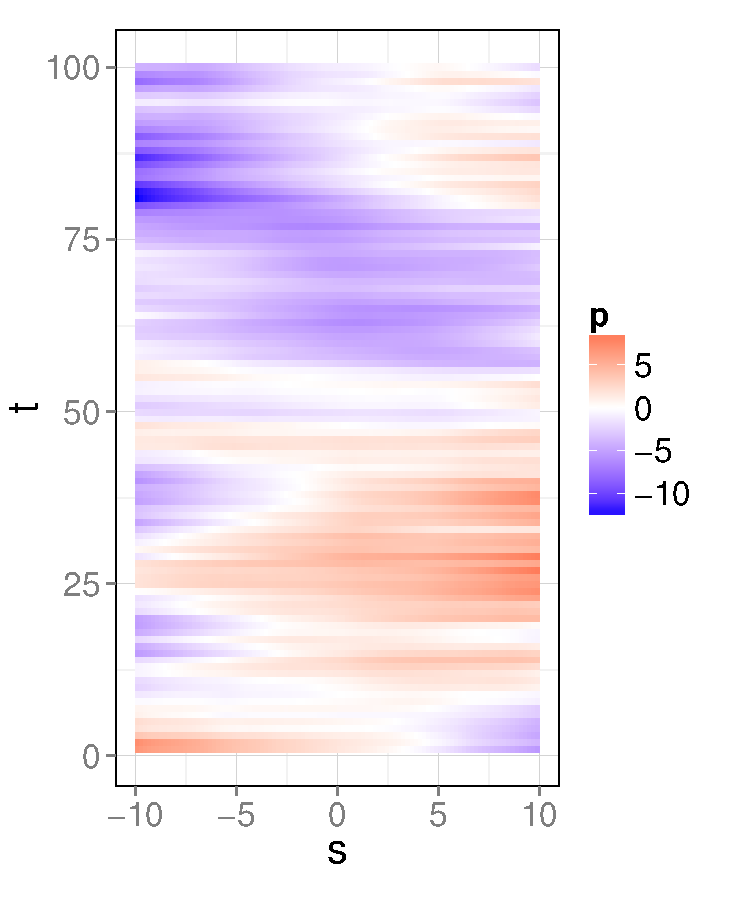
\includegraphics[width=\maxwidth]{figure/upsilon-plot2-1} 

\end{knitrout}
\end{center}
\caption{The parameter $\upsilon_t(s)$ simulated from the separable spatio-temporal process}
\label{fig:upsilon}
\end{figure}



\section{Process and observation simulation}

\subsection{Simulating the flux field}

Now that we have the parameters in place, we can simulate our dataset. We first re-set the seed to `1', then construct a semi-variogram with the parameters identical to those estimated from the Emissions data, before simulating our vector $\Yvec_f$:

\begin{knitrout}
\definecolor{shadecolor}{rgb}{0.969, 0.969, 0.969}\color{fgcolor}\begin{kframe}
\begin{alltt}
\hlcom{###------------------}
\hlcom{### Lognormal flux field}
\hlcom{###------------------}
\hlkwd{set.seed}\hlstd{(}\hlnum{1}\hlstd{)}
\hlstd{variogram_model} \hlkwb{<-} \hlkwd{vgm}\hlstd{(}\hlkwc{range} \hlstd{=} \hlnum{3.334}\hlstd{,}     \hlcom{# Construct spherical semi-variogram}
                       \hlkwc{nugget} \hlstd{=} \hlnum{0.00533}\hlstd{,}
                       \hlkwc{psill} \hlstd{=} \hlnum{0.80429}\hlstd{,}
                       \hlkwc{model}\hlstd{=} \hlstr{"Sph"}\hlstd{)}
\hlstd{S_f_log} \hlkwb{<-} \hlkwd{variogramLine}\hlstd{(variogram_model,} \hlcom{# Find covariance matrix Sigma_f}
                         \hlkwc{dist_vector} \hlstd{= sp}\hlopt{::}\hlkwd{spDists}\hlstd{(}\hlkwd{matrix}\hlstd{(s_axis),}
                                                 \hlkwd{matrix}\hlstd{(s_axis)),}
                          \hlkwc{covariance} \hlstd{=} \hlnum{TRUE}\hlstd{)}
\hlstd{mu_f_log} \hlkwb{<-} \hlkwd{matrix}\hlstd{(}\hlkwd{rep}\hlstd{(}\hlnum{5}\hlstd{,}\hlkwd{length}\hlstd{(s_axis)))}        \hlcom{# Construct mu_f}
\hlstd{Yf_sim} \hlkwb{<-} \hlkwd{exp}\hlstd{(mu_f_log} \hlopt{+} \hlkwd{t}\hlstd{(}\hlkwd{chol}\hlstd{(S_f_log))} \hlopt    \hlcom{# Simulate Y_f}
                \hlkwd{rnorm}\hlstd{(}\hlkwc{n} \hlstd{=} \hlkwd{length}\hlstd{(s_axis)))}
\hlstd{st_grid} \hlkwb{<-} \hlstd{st_grid} \hlopt                           \hlcom{# Append Y_f to data frame}
          \hlkwd{left_join}\hlstd{(}\hlkwd{data.frame}\hlstd{(}\hlkwc{s}\hlstd{=s_axis,}
                               \hlkwc{Yf} \hlstd{= Yf_sim))}
\end{alltt}


{\ttfamily\noindent\itshape\color{messagecolor}{\#\# Joining by: "{}s"{}}}\begin{alltt}
\hlkwa{if}\hlstd{(misspecification)  \{}               \hlcom{# If we are assuming misspecification}
    \hlstd{S_f_log} \hlkwb{<-} \hlkwd{diag}\hlstd{(}\hlkwd{diag}\hlstd{(S_f_log))}    \hlcom{# We over-write Sigma_f to be diagonal}
\hlstd{\}}
\end{alltt}
\end{kframe}
\end{knitrout}

\subsection{Simulating the mole fraction field}

Since the spatio-temporal discrepancy term can be hard to simulate from withour further approximations, we will just simulate it at the observation locations. Therefore, the mole fraction (excluding the discrepancy) is just a linear transformation of the flux field. For each space-time location we find the SRR between the whole domain (the source) and that point (the receptor) and multiply it by the the flux in the that gridcell:

\begin{knitrout}
\definecolor{shadecolor}{rgb}{0.969, 0.969, 0.969}\color{fgcolor}\begin{kframe}
\begin{alltt}
\hlcom{###------------------}
\hlcom{### Mole fraction field}
\hlcom{###------------------}
\hlcom{## Since we cannot put the discrepancy everywhere (too large), }
\hlcom{## we will just put it at the observation locations}
\hlstd{st_grid} \hlkwb{<-} \hlstd{st_grid} \hlopt
  \hlkwd{group_by}\hlstd{(t,s,p)} \hlopt \hlcom{# for each space-time location}
  \hlkwd{summarise}\hlstd{(}\hlkwc{Yf} \hlstd{= Yf,}  \hlcom{# find the mole-fraction by finding the SRR}
            \hlkwc{Ym} \hlstd{=} \hlkwd{sum}\hlstd{(}\hlkwd{b}\hlstd{(}\hlkwc{s} \hlstd{=s,} \hlkwc{u} \hlstd{= s_axis,}\hlkwc{p} \hlstd{= p)} \hlopt{*}
                       \hlstd{Yf_sim} \hlopt{*} \hlstd{ds))}
\end{alltt}
\end{kframe}
\end{knitrout}

\subsection{Simulating the observations}

We randomly choose \texttt{m\_obs} observations from the spatial grid (excluding the lower and upper 10 grid cells) and assume these are observed. We replace the 6-th observation location with $s = 0.3$ that will be used for validation.

\begin{knitrout}
\definecolor{shadecolor}{rgb}{0.969, 0.969, 0.969}\color{fgcolor}\begin{kframe}
\begin{alltt}
\hlcom{###------------------}
\hlcom{### Observations}
\hlcom{###------------------}
\hlkwa{if}\hlstd{(model} \hlopt \hlkwd{c}\hlstd{(}\hlstr{"full"}\hlstd{,}\hlstr{"diag"}\hlstd{)) \{}
      \hlstd{s_obs} \hlkwb{<-} \hlkwd{data.frame}\hlstd{(}\hlkwc{s} \hlstd{=} \hlkwd{sample}\hlstd{(s_axis[}\hlopt{-}\hlkwd{c}\hlstd{(}\hlnum{1}\hlopt{:}\hlnum{10}\hlstd{,(ns}\hlopt{-}\hlnum{10}\hlstd{)}\hlopt{:}\hlstd{ns)],}
                                     \hlkwc{size} \hlstd{= m_obs,}
                                     \hlkwc{replace}\hlstd{=F),}
                          \hlkwc{m} \hlstd{=} \hlnum{1}\hlopt{:}\hlstd{m_obs  )}
    \hlstd{new_obs} \hlkwb{<-} \hlnum{0.3}
    \hlstd{s_obs[}\hlnum{6}\hlstd{,]}\hlopt{$}\hlstd{s} \hlkwb{<-} \hlstd{new_obs}
\hlstd{\}} \hlkwa{else} \hlstd{\{}
  \hlstd{s_obs} \hlkwb{<-} \hlkwd{data.frame}\hlstd{(}\hlkwc{s} \hlstd{=} \hlkwd{sample}\hlstd{(s_axis,}\hlkwc{size} \hlstd{= m_obs,} \hlkwc{replace}\hlstd{=T),}
                      \hlkwc{m} \hlstd{=} \hlnum{1}\hlopt{:}\hlstd{m_obs)}
\hlstd{\}}
\end{alltt}
\end{kframe}
\end{knitrout}

Now we merge the observation data frame with the spaio-temporal grid and add the observation error, before sorting the data frame by time and space:

\begin{knitrout}
\definecolor{shadecolor}{rgb}{0.969, 0.969, 0.969}\color{fgcolor}\begin{kframe}
\begin{alltt}
\hlstd{s_obs} \hlkwb{<-} \hlstd{s_obs} \hlopt
            \hlkwd{left_join}\hlstd{(st_grid)} \hlopt
            \hlkwd{mutate}\hlstd{(}\hlkwc{z} \hlstd{= Ym} \hlopt{+} \hlkwd{rnorm}\hlstd{(}\hlkwc{n} \hlstd{=} \hlkwd{length}\hlstd{(Ym),}
                                  \hlkwc{sd} \hlstd{= sigma_eps_true))} \hlopt
            \hlkwd{arrange}\hlstd{(t,s)}
\end{alltt}


{\ttfamily\noindent\itshape\color{messagecolor}{\#\# Joining by: "{}s"{}}}\begin{alltt}
\hlstd{Qobs} \hlkwb{<-} \hlstd{sigma_eps_true}\hlopt{^}\hlstd{(}\hlopt{-}\hlnum{2}\hlstd{)} \hlopt{*} \hlkwd{.symDiagonal}\hlstd{(}\hlkwd{nrow}\hlstd{(s_obs))}
\end{alltt}
\end{kframe}
\end{knitrout}

To add the discrepancy, we first compuate the spatio-temporal covariance matrix at the observation (space-time) locations using the \texttt{corr\_zeta\_fn} function in the \texttt{atminv} package, find its Cholesky decomposition and then use it to simulate the discrepancy at the required locations. For when we have 2000 observations (\texttt{model = `full\_big'}) we find the covariance matrix at every space-time grid location and use assign the discrepancy to the observations at the grid level. The variable \texttt{C\_m} is a matrix that maps the location of the mole fraction observations to the mole fraction prediction grid. Note that for the `full' model this is just the $m \times m$ since with this model we are choosing not predicting the mole fraction in every grid cell:

\begin{knitrout}
\definecolor{shadecolor}{rgb}{0.969, 0.969, 0.969}\color{fgcolor}\begin{kframe}
\begin{alltt}
\hlcom{## Now add the discrepancy}
\hlkwa{if}\hlstd{(model} \hlopt \hlkwd{c}\hlstd{(}\hlstr{"full"}\hlstd{,}\hlstr{"diag"}\hlstd{)) \{}

    \hlstd{corr_zeta_true} \hlkwb{<-} \hlkwd{corr_zeta_fn}\hlstd{(s_obs}\hlopt{$}\hlstd{s[}\hlnum{1}\hlopt{:}\hlstd{m_obs],}
                                   \hlstd{t_axis,}
                                   \hlstd{theta_t_true,}
                                   \hlstd{theta_s_true)}
    \hlstd{S_zeta_true} \hlkwb{<-} \hlstd{sigma_zeta_true}\hlopt{^}\hlnum{2} \hlopt{*} \hlstd{corr_zeta_true}
    \hlstd{chol_S_zeta_true} \hlkwb{<-} \hlkwd{chol}\hlstd{(S_zeta_true)}

    \hlstd{s_obs} \hlkwb{<-} \hlstd{s_obs} \hlopt
      \hlkwd{mutate}\hlstd{(}\hlkwc{dis} \hlstd{=} \hlkwd{t}\hlstd{(chol_S_zeta_true)} \hlopt  \hlkwd{rnorm}\hlstd{(}\hlkwc{n} \hlstd{=} \hlkwd{nrow}\hlstd{(s_obs)),}
             \hlkwc{z} \hlstd{= z} \hlopt{+} \hlstd{dis)}

    \hlstd{C_m} \hlkwb{<-} \hlkwd{.symDiagonal}\hlstd{(}\hlkwd{nrow}\hlstd{(s_obs))}
\hlstd{\}} \hlkwa{else if}\hlstd{(model} \hlopt{==} \hlstr{"full_big"}\hlstd{) \{}

    \hlstd{corr_s_mat} \hlkwb{<-} \hlkwa{function}\hlstd{(}\hlkwc{theta_s}\hlstd{)} \hlkwd{corr_s}\hlstd{(}\hlkwc{s} \hlstd{= s_axis,}\hlkwc{theta_s} \hlstd{= theta_s)}
    \hlstd{corr_t_mat} \hlkwb{<-} \hlkwa{function}\hlstd{(}\hlkwc{theta_t}\hlstd{)} \hlkwd{corr_t}\hlstd{(}\hlkwc{t} \hlstd{= t_axis,}\hlkwc{theta_t} \hlstd{= theta_t)}
    \hlstd{d_corr_s_mat} \hlkwb{<-} \hlkwa{function}\hlstd{(}\hlkwc{theta_s}\hlstd{)} \hlkwd{d_corr_s}\hlstd{(}\hlkwc{s} \hlstd{= s_axis,}\hlkwc{theta_s} \hlstd{= theta_s)}
    \hlstd{d_corr_t_mat} \hlkwb{<-} \hlkwa{function}\hlstd{(}\hlkwc{theta_t}\hlstd{)} \hlkwd{d_corr_t}\hlstd{(}\hlkwc{t} \hlstd{= t_axis,}\hlkwc{theta_t} \hlstd{= theta_t)}

    \hlstd{C_idx} \hlkwb{<-} \hlstd{st_grid} \hlopt
      \hlkwd{as.data.frame}\hlstd{()} \hlopt
      \hlkwd{select}\hlstd{(s,t)} \hlopt
      \hlkwd{mutate}\hlstd{(}\hlkwc{n} \hlstd{=} \hlnum{1}\hlopt{:}\hlkwd{nrow}\hlstd{(st_grid))} \hlopt
      \hlkwd{left_join}\hlstd{(s_obs,.)}

    \hlstd{C_m} \hlkwb{<-} \hlkwd{sparseMatrix}\hlstd{(}\hlkwc{i}\hlstd{=}\hlnum{1}\hlopt{:}\hlkwd{nrow}\hlstd{(C_idx),}
                        \hlkwc{j} \hlstd{= C_idx}\hlopt{$}\hlstd{n,}
                        \hlkwc{x}\hlstd{=}\hlnum{1}\hlstd{,}
                        \hlkwc{dims}\hlstd{=}\hlkwd{c}\hlstd{(}\hlkwd{nrow}\hlstd{(s_obs),}\hlkwd{nrow}\hlstd{(st_grid)))}

    \hlstd{chol_S_zeta_true} \hlkwb{<-}  \hlstd{sigma_zeta_true} \hlopt{*}
                              \hlkwd{kronecker}\hlstd{(}\hlkwd{chol}\hlstd{(}\hlkwd{corr_t_mat}\hlstd{(theta_t_true)),}
                                        \hlkwd{chol}\hlstd{(}\hlkwd{corr_s_mat}\hlstd{(theta_s_true)))}

    \hlstd{s_obs} \hlkwb{<-} \hlstd{s_obs} \hlopt
        \hlkwd{mutate}\hlstd{(}\hlkwc{dis} \hlstd{=} \hlkwd{as.vector}\hlstd{(C_m} \hlopt
                                 \hlstd{(}\hlkwd{t}\hlstd{(chol_S_zeta_true)} \hlopt
                                    \hlkwd{rnorm}\hlstd{(}\hlkwc{n} \hlstd{= ns}\hlopt{*}\hlstd{nt))),}
               \hlkwc{z} \hlstd{= z} \hlopt{+} \hlstd{dis)}
\hlstd{\}}
\end{alltt}
\end{kframe}
\end{knitrout}



\subsection{Illustrative plots}

Here we provide the code for generating the two plots in the paper (Figure 3). The first, in Figure \ref{fig:YfYm}, shows the average mole fraction and the flux field superimposed:

\begin{knitrout}
\definecolor{shadecolor}{rgb}{0.969, 0.969, 0.969}\color{fgcolor}\begin{kframe}
\begin{alltt}
\hlkwa{if}\hlstd{(model} \hlopt{==} \hlstr{"full"}\hlstd{) \{}
    \hlstd{X} \hlkwb{<-} \hlkwd{group_by}\hlstd{(st_grid,s)} \hlopt
        \hlkwd{summarise}\hlstd{(}\hlkwc{Yf} \hlstd{= Yf[}\hlnum{1}\hlstd{],}\hlkwc{Ym_av} \hlstd{=} \hlkwd{mean}\hlstd{(Ym))} \hlopt
        \hlkwd{gather}\hlstd{(process,value,}\hlopt{-}\hlstd{s)}
    \hlstd{g} \hlkwb{<-} \hlkwd{LinePlotTheme}\hlstd{()} \hlopt{+}
          \hlkwd{geom_line}\hlstd{(}\hlkwc{data}\hlstd{=}\hlkwd{subset}\hlstd{(X,}\hlopt{!}\hlstd{(s}\hlopt{==}\hlstd{new_obs)),}
                    \hlkwd{aes}\hlstd{(}\hlkwc{x}\hlstd{=s,}\hlkwc{y}\hlstd{=value,}\hlkwc{linetype}\hlstd{=}\hlkwd{as.factor}\hlstd{(process)))}\hlopt{+}
          \hlkwd{geom_segment}\hlstd{(}\hlkwc{data}\hlstd{=s_obs[}\hlnum{1}\hlopt{:}\hlnum{5}\hlstd{,],}
                       \hlkwd{aes}\hlstd{(}\hlkwc{x}\hlstd{=s,} \hlkwc{xend}\hlstd{=s,} \hlkwc{y} \hlstd{=} \hlnum{0}\hlstd{,} \hlkwc{yend} \hlstd{=} \hlnum{50}\hlstd{),}
                        \hlkwc{arrow}\hlstd{=}\hlkwd{arrow}\hlstd{(}\hlkwc{length}\hlstd{=}\hlkwd{unit}\hlstd{(}\hlnum{0.1}\hlstd{,}\hlstr{"cm"}\hlstd{)))} \hlopt{+}
        \hlkwd{ylab}\hlstd{(}\hlstr{""}\hlstd{)} \hlopt{+}
        \hlkwd{scale_linetype_discrete}\hlstd{(}\hlkwc{guide}\hlstd{=}\hlkwd{guide_legend}\hlstd{(}\hlkwc{title}\hlstd{=}\hlstr{"process"}\hlstd{),}
                                \hlkwc{labels}\hlstd{=}\hlkwd{c}\hlstd{(}\hlstr{"Yf (g/s/degree)"}\hlstd{,}\hlstr{"Ym (ppb)"}\hlstd{))} \hlopt{+}
        \hlkwd{xlab}\hlstd{(}\hlstr{"s (degrees)"}\hlstd{)}
    \hlkwd{ggsave}\hlstd{(g,}\hlkwc{filename} \hlstd{=} \hlstr{"../../Sim_plot.png"}\hlstd{,}\hlkwc{width}\hlstd{=}\hlnum{10}\hlstd{,}\hlkwc{height}\hlstd{=}\hlnum{4}\hlstd{)}
\hlstd{\}}
\end{alltt}
\end{kframe}
\end{knitrout}

\begin{figure}
\begin{center}
\begin{knitrout}
\definecolor{shadecolor}{rgb}{0.969, 0.969, 0.969}\color{fgcolor}\begin{kframe}
\begin{alltt}
\hlkwd{print}\hlstd{(g)}
\end{alltt}
\end{kframe}
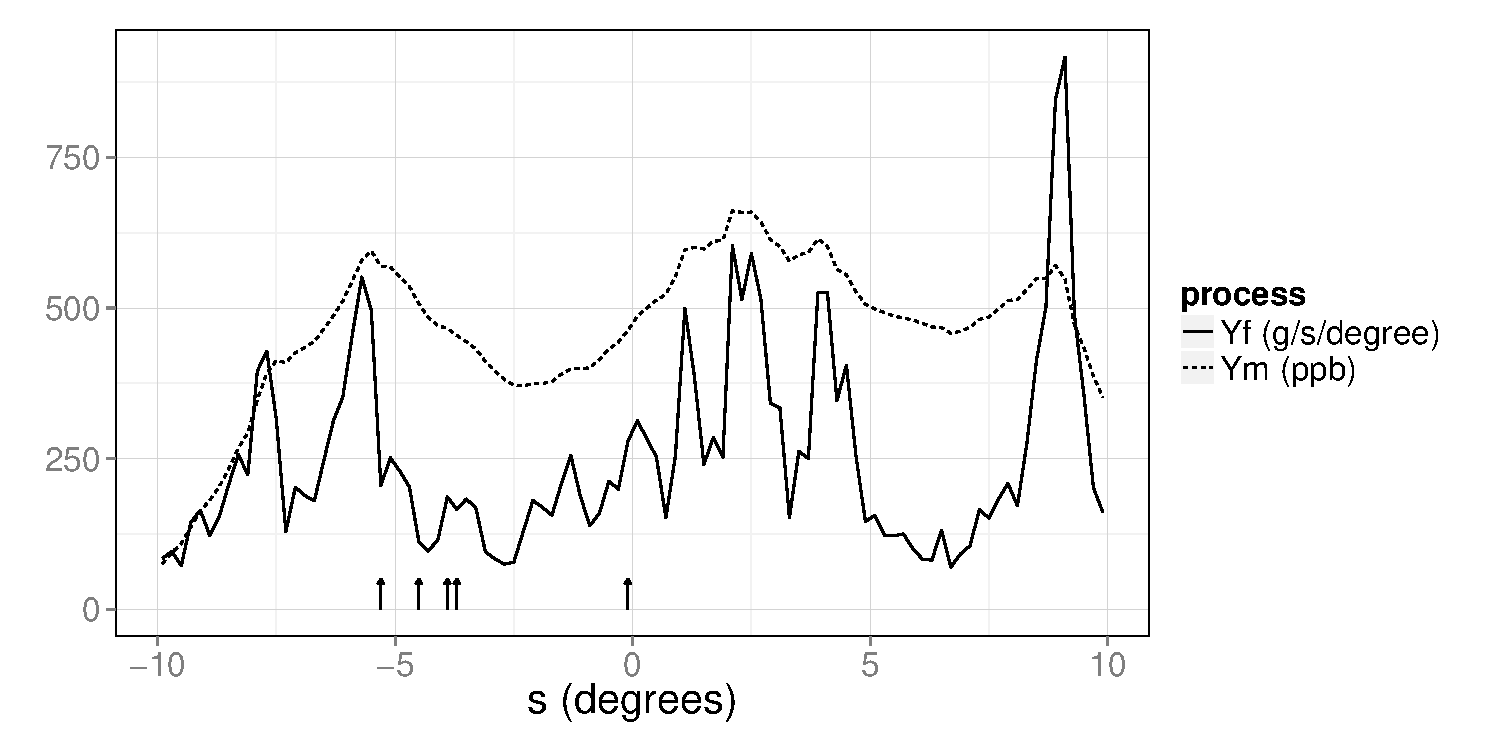
\includegraphics[width=\maxwidth]{figure/YfYm-plot-1} 

\end{knitrout}
\end{center}
\caption{A sample realisation of the flux field (solid line), the resulting time-averaged mole-fraction field (dashed line) and the five observation locations (arrows).}
\label{fig:YfYm}
\end{figure}






The second, in Figure \ref{fig:B}, shows the SRR at each observation location:

\begin{knitrout}
\definecolor{shadecolor}{rgb}{0.969, 0.969, 0.969}\color{fgcolor}\begin{kframe}
\begin{alltt}
\hlkwa{if}\hlstd{(model} \hlopt \hlkwd{c}\hlstd{(}\hlstr{"full"}\hlstd{,}\hlstr{"diag"}\hlstd{)) \{}
  \hlstd{df_for_B} \hlkwb{<-} \hlstd{s_obs}
\hlstd{\}} \hlkwa{else} \hlstd{\{}
  \hlstd{df_for_B} \hlkwb{<-} \hlstd{st_grid}
\hlstd{\}}

\hlcom{# TRUE B}
\hlstd{B_true} \hlkwb{<-} \hlstd{plyr}\hlopt{::}\hlkwd{ddply}\hlstd{(df_for_B,}\hlkwd{c}\hlstd{(}\hlstr{"t"}\hlstd{,}\hlstr{"s"}\hlstd{),}\hlkwa{function}\hlstd{(}\hlkwc{df}\hlstd{) \{}
  \hlstd{b} \hlkwb{=} \hlkwd{b}\hlstd{(}\hlkwc{s}\hlstd{=df}\hlopt{$}\hlstd{s[}\hlnum{1}\hlstd{],}\hlkwc{u}\hlstd{=s_axis,}\hlkwc{p}\hlstd{=df}\hlopt{$}\hlstd{p[}\hlnum{1}\hlstd{])\})} \hlopt
  \hlkwd{select}\hlstd{(}\hlopt{-}\hlstd{s,}\hlopt{-}\hlstd{t)} \hlopt
  \hlkwd{as.matrix}\hlstd{()}\hlopt{*}\hlstd{ds}

\hlstd{B} \hlkwb{<-} \hlstd{B_true}
\hlkwa{if}\hlstd{(model} \hlopt{==} \hlstr{"sparse"}\hlstd{) \{}
  \hlstd{B} \hlkwb{<-} \hlkwd{as}\hlstd{(B,}\hlstr{"dgCMatrix"}\hlstd{)}
\hlstd{\}}

\hlstd{B_true_df} \hlkwb{<-} \hlstd{plyr}\hlopt{::}\hlkwd{ddply}\hlstd{(df_for_B,}\hlkwd{c}\hlstd{(}\hlstr{"t"}\hlstd{,}\hlstr{"s"}\hlstd{),}\hlkwa{function}\hlstd{(}\hlkwc{df}\hlstd{) \{}
  \hlstd{b} \hlkwb{=} \hlkwd{b}\hlstd{(}\hlkwc{s}\hlstd{=df}\hlopt{$}\hlstd{s[}\hlnum{1}\hlstd{],}\hlkwc{u}\hlstd{=s_axis,}\hlkwc{p}\hlstd{=df}\hlopt{$}\hlstd{p[}\hlnum{1}\hlstd{])\})} \hlopt
  \hlkwd{gather}\hlstd{(s_grid,b,}\hlopt{-}\hlstd{t,}\hlopt{-}\hlstd{s)} \hlopt
  \hlkwd{separate}\hlstd{(s_grid,} \hlkwc{into} \hlstd{=} \hlkwd{c}\hlstd{(}\hlstr{"V"}\hlstd{,}\hlstr{"s_fine"}\hlstd{),}\hlkwc{sep}\hlstd{=}\hlstr{"V"}\hlstd{)} \hlopt
  \hlkwd{select}\hlstd{(}\hlopt{-}\hlstd{V)} \hlopt
  \hlkwd{mutate}\hlstd{(}\hlkwc{s_fine} \hlstd{=} \hlkwd{round}\hlstd{(s_axis[}\hlkwd{as.numeric}\hlstd{(s_fine)],}\hlnum{1}\hlstd{))}\hlcom{# %>%}
\hlcom{#left_join(model_pred_em,by = c("t","s","s_fine"))}


\hlkwa{if}\hlstd{(model} \hlopt{==} \hlstr{"full"}\hlstd{) \{}
  \hlcom{## Plot the source-receptor relationship at each observation}

  \hlcom{## The following code uses colours and shows the SRR on one plot  }
  \hlcom{#   B_plot <- LinePlotTheme() + }
  \hlcom{#             geom_tile(data=subset(B_true_df ,b>0),}
  \hlcom{#                       aes(x=s_fine,y=t,fill=as.factor(s),alpha=b)) +}
  \hlcom{#     scale_alpha_continuous(range=c(0,1)) + xlab("u") +}
  \hlcom{#     scale_fill_discrete(guide=guide_legend(title="s")) +}
  \hlcom{#     coord_fixed(xlim=c(-10,10),ratio = 0.2)}

  \hlcom{## The following code shows one SRR per plot  }
  \hlstd{B_plot} \hlkwb{<-} \hlkwd{LinePlotTheme}\hlstd{()} \hlopt{+}
    \hlkwd{geom_tile}\hlstd{(}\hlkwc{data}\hlstd{=}\hlkwd{subset}\hlstd{(B_true_df,b}\hlopt{>}\hlnum{0} \hlopt{& !}\hlstd{(s}\hlopt{==}\hlstd{new_obs)),}
              \hlkwd{aes}\hlstd{(}\hlkwc{x}\hlstd{=s_fine,}\hlkwc{y}\hlstd{=t,}\hlkwc{alpha}\hlstd{=b),}\hlkwc{fill}\hlstd{=}\hlstr{"black"}\hlstd{)} \hlopt{+}
    \hlkwd{scale_alpha_continuous}\hlstd{(}\hlkwc{guide}\hlstd{=}\hlkwd{guide_legend}\hlstd{(}\hlkwc{title}\hlstd{=}\hlstr{"s/ng"}\hlstd{))} \hlopt{+}
    \hlkwd{scale_y_reverse}\hlstd{()}\hlopt{+}
    \hlkwd{scale_fill_discrete}\hlstd{(}\hlkwc{guide}\hlstd{=}\hlkwd{guide_legend}\hlstd{(}\hlkwc{title}\hlstd{=}\hlstr{"s"}\hlstd{))} \hlopt{+}
    \hlkwd{coord_fixed}\hlstd{(}\hlkwc{xlim}\hlstd{=}\hlkwd{c}\hlstd{(}\hlopt{-}\hlnum{10}\hlstd{,}\hlnum{10}\hlstd{),}\hlkwc{ratio} \hlstd{=} \hlnum{0.5}\hlstd{)}  \hlopt{+}
    \hlkwd{facet_grid}\hlstd{(}\hlopt{~}\hlstd{s)} \hlopt{+}
    \hlkwd{theme}\hlstd{(}\hlkwc{panel.margin} \hlstd{=} \hlkwd{unit}\hlstd{(}\hlnum{1.5}\hlstd{,} \hlstr{"lines"}\hlstd{))} \hlopt{+}
    \hlkwd{xlab}\hlstd{(}\hlstr{"u (degrees)"}\hlstd{)} \hlopt{+}
    \hlkwd{ylab}\hlstd{(}\hlstr{"t (2 h steps)"}\hlstd{)}
  \hlkwd{ggsave}\hlstd{(}\hlkwc{filename} \hlstd{=} \hlstr{"../../B_plot.png"}\hlstd{,}\hlkwc{width}\hlstd{=}\hlnum{12}\hlstd{)}
\hlstd{\}}
\end{alltt}
\end{kframe}
\end{knitrout}

\begin{figure}
\begin{center}
\begin{knitrout}
\definecolor{shadecolor}{rgb}{0.969, 0.969, 0.969}\color{fgcolor}\begin{kframe}
\begin{alltt}
\hlkwd{print}\hlstd{(B_plot)}
\end{alltt}
\end{kframe}
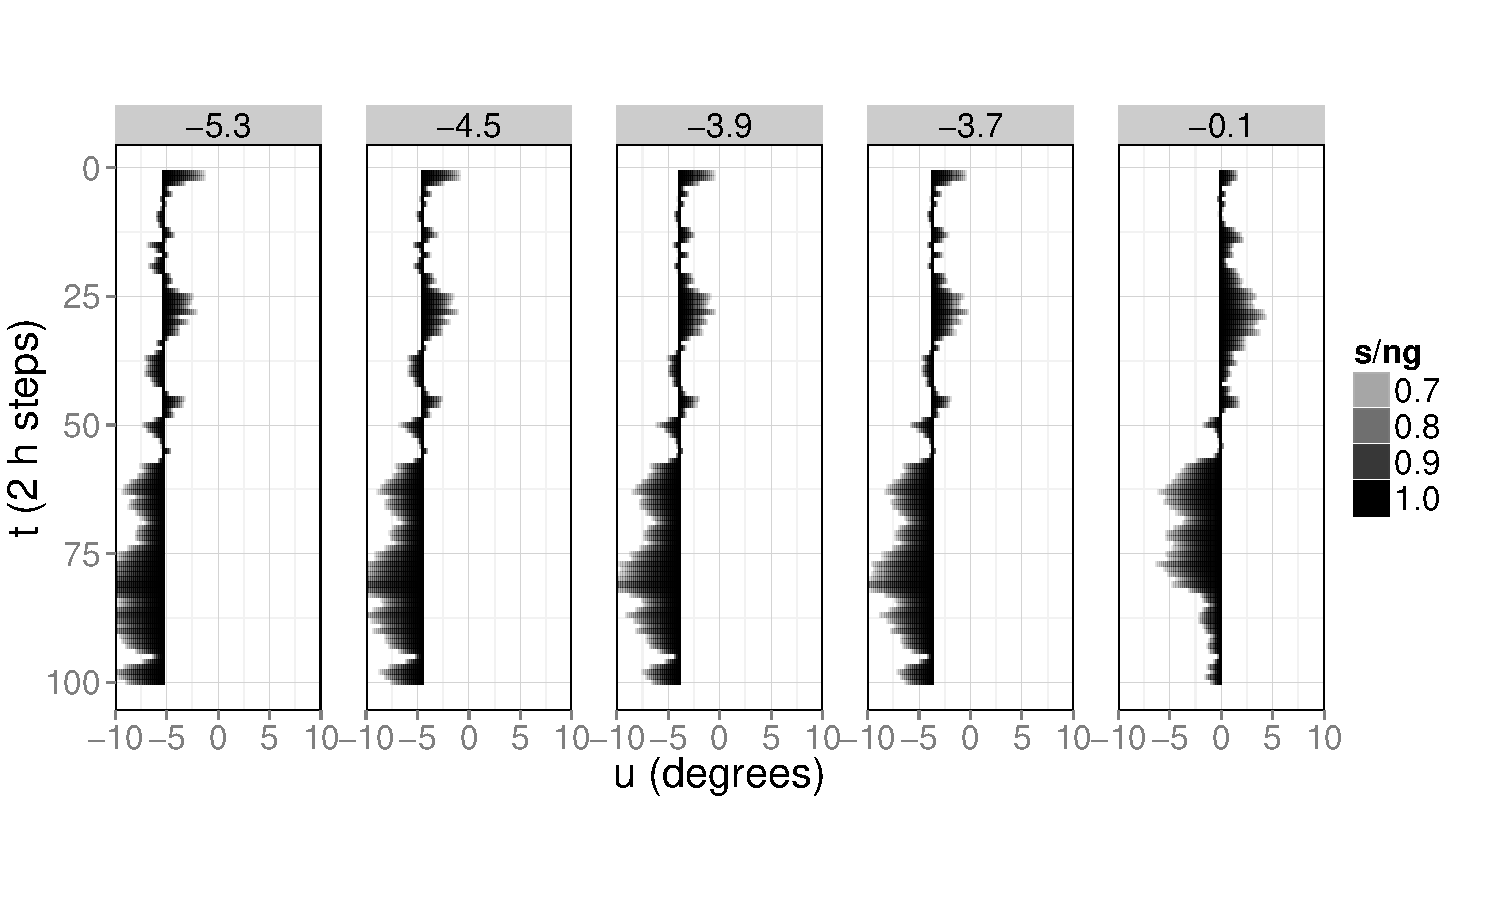
\includegraphics[width=\maxwidth]{figure/B-plot-1} 

\end{knitrout}
\end{center}
\caption{ The source-receptor relationship $b_t(s,u)$ synthesised at five observation locations $s \in D^O_m = \{-5.3^\circ, -4.5^\circ,-3.9^\circ,-3.7^\circ,-0.1^\circ \}$. Note that $b_t(s,u) = 0$ for $u > 4.3$}
\label{fig:B}
\end{figure}






\section{EM algorithm}

In this section we show the code for carrying inference on the bivariate field $(\Yvec_f,\Yvec_m)'$. We first compute the mean flux density, which we will then also use as the initial value for the conditional expectation of $\Yvec_f$ in the gradient descent:


\begin{knitrout}
\definecolor{shadecolor}{rgb}{0.969, 0.969, 0.969}\color{fgcolor}\begin{kframe}
\begin{alltt}
\hlstd{mu_f} \hlkwb{<-} \hlkwd{matrix}\hlstd{(}\hlkwd{exp}\hlstd{(mu_f_log} \hlopt{+} \hlnum{0.5}\hlopt{*}\hlkwd{diag}\hlstd{(S_f_log)))}
\end{alltt}
\end{kframe}
\end{knitrout}

We then set the settings for the Laplace approximation. These vary accoring to the model being used. For the model `full', we alter the matrices so that the validation point is excluded. :

\begin{knitrout}
\definecolor{shadecolor}{rgb}{0.969, 0.969, 0.969}\color{fgcolor}\begin{kframe}
\begin{alltt}
\hlcom{###-----------------------------------------------------}
\hlcom{### Laplace method -- use with caution because of mode close to zero}
\hlcom{###-----------------------------------------------------}
\hlstd{n_EM} \hlkwb{<-} \hlnum{100}

\hlkwa{if}\hlstd{(model} \hlopt{==} \hlstr{"full"}\hlstd{) \{}
  \hlstd{s_mol} \hlkwb{=} \hlstd{s_obs}\hlopt{$}\hlstd{s[}\hlnum{1}\hlopt{:}\hlstd{m_obs]}         \hlcom{# prediction locs for mol fraction}
  \hlstd{Y_init} \hlkwb{=} \hlkwd{c}\hlstd{(mu_f,s_obs}\hlopt{$}\hlstd{z)}         \hlcom{# initial expectation value for Y}
  \hlstd{theta_init} \hlkwb{=} \hlkwd{c}\hlstd{(}\hlnum{1000}\hlstd{,}\hlnum{0.2}\hlstd{,}\hlnum{0.2}\hlstd{)}     \hlcom{# initial parameter vector}
                                   \hlcom{# where theta = [sigma_zeta^2, theta_t, theat_s]}

  \hlcom{# Keep station out for validation}
  \hlstd{rm_idx} \hlkwb{<-} \hlkwd{seq}\hlstd{(}\hlnum{6}\hlstd{,}\hlkwd{nrow}\hlstd{(C_m),}\hlkwc{by}\hlstd{=}\hlnum{6}\hlstd{)} \hlcom{# index to be removed}
  \hlstd{s_obs_old} \hlkwb{<-} \hlstd{s_obs}              \hlcom{# save old observation location data frame}
  \hlstd{s_obs} \hlkwb{<-} \hlstd{s_obs[}\hlopt{-}\hlstd{rm_idx,]}        \hlcom{# new observation data frame}
  \hlstd{C_m} \hlkwb{<-} \hlstd{C_m[}\hlopt{-}\hlstd{rm_idx,]}            \hlcom{# new incidence matrix}
  \hlstd{Qobs} \hlkwb{<-} \hlstd{Qobs[}\hlopt{-}\hlstd{rm_idx,}\hlopt{-}\hlstd{rm_idx]}   \hlcom{# new (observation) precision matrix}

\hlstd{\}} \hlkwa{else if} \hlstd{(model} \hlopt{==} \hlstr{"full_big"}\hlstd{) \{}
    \hlstd{s_mol} \hlkwb{=} \hlstd{s_axis}                \hlcom{# prediction locs for mol fraction}
    \hlstd{Y_init} \hlkwb{=} \hlkwd{c}\hlstd{(mu_f,st_grid}\hlopt{$}\hlstd{Ym)}   \hlcom{# initial expectation value for Y}
    \hlstd{theta_init} \hlkwb{=} \hlkwd{c}\hlstd{(}\hlnum{1000}\hlstd{,}\hlnum{0.2}\hlstd{,}\hlnum{0.2}\hlstd{)}  \hlcom{# initial parameter vector}
                                  \hlcom{# where theta = [sigma_zeta^2, theta_t, theat_s]}
\hlstd{\}}
\end{alltt}
\end{kframe}
\end{knitrout}



We are now ready to call the main function of the \texttt{EM\_alg} package, which returns a function that can be iterated. The inputs to this function are given in-line:


\begin{knitrout}
\definecolor{shadecolor}{rgb}{0.969, 0.969, 0.969}\color{fgcolor}\begin{kframe}
\begin{alltt}
\hlstd{EM_alg} \hlkwb{<-} \hlkwd{EM}\hlstd{(}\hlkwc{s_obs} \hlstd{= s_obs,}                  \hlcom{# observation data frame}
        \hlkwc{C_m} \hlstd{= C_m,}                           \hlcom{# incidence matrix}
        \hlkwc{Qobs} \hlstd{= Qobs,}                         \hlcom{# observation precision matrix}
        \hlkwc{B} \hlstd{= B,}                               \hlcom{# SRR matrix}
        \hlkwc{t_mol} \hlstd{= t_axis,}                      \hlcom{# time prediction locs}
        \hlkwc{s_mol} \hlstd{=} \hlkwd{matrix}\hlstd{(s_mol),}               \hlcom{# spatial prediction locs}
        \hlkwc{S_f_log} \hlstd{= S_f_log,}                   \hlcom{# cov. matrix of log(Yf)}
        \hlkwc{mu_f_log} \hlstd{= mu_f_log,}                 \hlcom{# expectation of log(Yf)}
        \hlkwc{Yf_thresh} \hlstd{=} \hlnum{1e-4}\hlstd{,}                    \hlcom{# drop nodes with Yf < 1e-4}
        \hlkwc{Y_init} \hlstd{=  Y_init,}                    \hlcom{# initialise Yf}
        \hlkwc{theta_init} \hlstd{= theta_init,}             \hlcom{# initialise theta}
        \hlkwc{ind} \hlstd{=} \hlkwd{which}\hlstd{(}\hlopt{!}\hlstd{(}\hlkwd{colSums}\hlstd{(B)} \hlopt{==} \hlnum{0}\hlstd{)),}     \hlcom{# only consider indices with SRR>0}
        \hlkwc{n_EM} \hlstd{= n_EM,}                         \hlcom{# number of EM iterations}
        \hlkwc{model} \hlstd{= model)}                       \hlcom{# model we are using}
\end{alltt}
\end{kframe}
\end{knitrout}

To iterate the E- and M-steps we simply put the returned function in a loop, and indicate the maximum numer of gradient descents to carry out in the E- and M- steps. In this case we are going to limit the number of M-steps to 50. We also allow for a variable \texttt{fine\_tune\_E} that indicates on which iteration to carry out a second gradient descent at a higher convergence tolerance. This is particularly useful when the Hessian computed at `convergence' is not positive definite due to the tolerance used. 

\begin{knitrout}
\definecolor{shadecolor}{rgb}{0.969, 0.969, 0.969}\color{fgcolor}\begin{kframe}
\begin{alltt}
\hlstd{filename} \hlkwb{<-} \hlkwd{paste0}\hlstd{(model,}\hlstr{"_misspec_"}\hlstd{,misspecification,}\hlstr{".rda"}\hlstd{)}
\hlkwa{if}\hlstd{(load_results) \{}
  \hlkwd{load}\hlstd{(}\hlkwd{system.file}\hlstd{(}\hlstr{"extdata"}\hlstd{,filename,} \hlkwc{package} \hlstd{=} \hlstr{"atminv"}\hlstd{))}
\hlstd{\}} \hlkwa{else} \hlstd{\{}
  \hlkwa{for}\hlstd{(i} \hlkwa{in} \hlnum{1}\hlopt{:}\hlstd{(n_EM}\hlopt{-}\hlnum{2}\hlstd{)) \{}
    \hlstd{X} \hlkwb{<-} \hlkwd{EM_alg}\hlstd{(}\hlkwc{max_E_it} \hlstd{=} \hlnum{1e6}\hlstd{,}
                \hlkwc{max_M_it} \hlstd{=} \hlnum{50}\hlstd{,}
                \hlkwc{fine_tune_E} \hlstd{= (i}\hlopt{==}\hlnum{0}\hlstd{))}
  \hlstd{\}}
\hlstd{\}}
\end{alltt}
\end{kframe}
\end{knitrout}

The final parameter estimates are given by
\begin{knitrout}
\definecolor{shadecolor}{rgb}{0.969, 0.969, 0.969}\color{fgcolor}\begin{kframe}
\begin{alltt}
\hlstd{X}\hlopt{$}\hlstd{theta[,n_EM}\hlopt{-}\hlnum{1}\hlstd{]}
\end{alltt}
\begin{verbatim}
## [1] 1964.9329277    0.7135804    0.7721958
\end{verbatim}
\end{kframe}
\end{knitrout}


\section{HMC sampler}

In this section we show the code for the HMC sampler, that fixes the parameters found using the EM algorithm above. We first compute the covariance matrix:

\begin{knitrout}
\definecolor{shadecolor}{rgb}{0.969, 0.969, 0.969}\color{fgcolor}\begin{kframe}
\begin{alltt}
\hlkwa{if}\hlstd{(model} \hlopt{==} \hlstr{"full"}\hlstd{) \{}
  \hlstd{corr_zeta} \hlkwb{<-} \hlkwd{corr_zeta_fn}\hlstd{(}\hlkwd{c}\hlstd{(s_obs}\hlopt{$}\hlstd{s[}\hlnum{1}\hlopt{:}\hlstd{(m_obs}\hlopt{-}\hlnum{1}\hlstd{)],new_obs),t_axis,X}\hlopt{$}\hlstd{theta[}\hlnum{2}\hlstd{,n_EM],X}\hlopt{$}\hlstd{theta[}\hlnum{3}\hlstd{,n_EM])}
  \hlstd{S_zeta} \hlkwb{<-} \hlstd{X}\hlopt{$}\hlstd{theta[}\hlnum{1}\hlstd{,n_EM]} \hlopt{*} \hlstd{corr_zeta}
  \hlstd{Q_zeta} \hlkwb{<-} \hlkwd{chol2inv}\hlstd{(}\hlkwd{chol}\hlstd{(S_zeta))}
\hlstd{\}}
\end{alltt}
\end{kframe}
\end{knitrout}



Now we formulate the equations required for the log-likelihood and the gradient of the log-likelihood of $\Yvec_f$. These are provided in the helper function \texttt{Yf\_marg\_approx\_fns} and its arguments are explained in-line.

\begin{knitrout}
\definecolor{shadecolor}{rgb}{0.969, 0.969, 0.969}\color{fgcolor}\begin{kframe}
\begin{alltt}
\hlstd{lap2} \hlkwb{<-} \hlkwd{Yf_marg_approx_fns}\hlstd{(}\hlkwc{s} \hlstd{= s_obs,}            \hlcom{# obs. locations}
                           \hlkwc{C_m} \hlstd{= C_m,}            \hlcom{# incidence matrix}
                           \hlkwc{Qobs} \hlstd{= Qobs,}          \hlcom{# obs. precision matrix}
                           \hlkwc{B} \hlstd{= B,}                \hlcom{# SRR matrix}
                           \hlkwc{S_zeta} \hlstd{= S_zeta,}      \hlcom{# Sigma_zeta}
                           \hlkwc{mu_f_log} \hlstd{= mu_f_log,}  \hlcom{# expectation of log(Y_f)}
                           \hlkwc{S_f_log} \hlstd{= S_f_log,}    \hlcom{# covariance of log(Y_f)}
                           \hlkwc{ind}\hlstd{=X}\hlopt{$}\hlstd{ind)}            \hlcom{# only consider indices with SRR>0}
\end{alltt}
\end{kframe}
\end{knitrout}

Next, we set some parameters for the sampler. We set the number of steps per sample $L = 10$, the number of samples $N = 10000$, and the step-size $\Delta \in [0.066,0.068]$ (below denoted as `eps\_gen'). Other variables are defined in-line:

\begin{knitrout}
\definecolor{shadecolor}{rgb}{0.969, 0.969, 0.969}\color{fgcolor}\begin{kframe}
\begin{alltt}
\hlstd{M} \hlkwb{<-} \hlkwd{diag}\hlstd{(}\hlnum{1}\hlopt{/}\hlstd{(X}\hlopt{$}\hlstd{lap_approx}\hlopt{$}\hlstd{Yf}\hlopt{^}\hlnum{2}\hlstd{))} \hlcom{# scaling matrix: puts variables on same scale}

\hlkwa{if}\hlstd{(model} \hlopt{==} \hlstr{"full"}\hlstd{)\{}             \hlcom{# Function for generating Delta}
  \hlstd{eps_gen} \hlkwb{<-} \hlkwa{function}\hlstd{()}
    \hlkwd{runif}\hlstd{(}\hlkwc{n}\hlstd{=}\hlnum{1}\hlstd{,}
          \hlkwc{min} \hlstd{=} \hlnum{0.066}\hlstd{,}
          \hlkwc{max} \hlstd{=} \hlnum{0.068}\hlstd{)}
\hlstd{\}} \hlkwa{else if} \hlstd{(model} \hlopt{==}\hlstr{"diag"}\hlstd{) \{}
  \hlstd{eps_gen} \hlkwb{<-} \hlkwa{function}\hlstd{()}
    \hlkwd{runif}\hlstd{(}\hlkwc{n}\hlstd{=}\hlnum{1}\hlstd{,}
          \hlkwc{min} \hlstd{=} \hlnum{0.0065}\hlstd{,}
          \hlkwc{max} \hlstd{=} \hlnum{0.0067}\hlstd{)}
\hlstd{\}}
\hlstd{L} \hlkwb{<-} \hlnum{10L}                   \hlcom{# step-size}
\hlstd{N} \hlkwb{<-} \hlnum{100}                 \hlcom{# number of samples}
\hlstd{q} \hlkwb{<-} \hlkwd{matrix}\hlstd{(}\hlnum{0}\hlstd{,}\hlkwd{nrow}\hlstd{(M),N)}   \hlcom{# matrix for storing samples}
\hlstd{qsamp} \hlkwb{<-} \hlstd{X}\hlopt{$}\hlstd{lap_approx}\hlopt{$}\hlstd{Yf}   \hlcom{# first sample}
\hlstd{dither} \hlkwb{<-} \hlstd{i} \hlkwb{<-} \hlstd{count} \hlkwb{<-} \hlnum{1}  \hlcom{# no dithering, initialise counts}

\hlcom{# if(!(N==10000) & cache_results) }
\hlcom{#   stop("Cannot cache unless N =10000")}
\end{alltt}
\end{kframe}
\end{knitrout}


The sampler is set up using the function \texttt{sampler} in the \texttt{hmc} package. We set a lower limit of 0; no samples less or equal to zero are allowed:

\begin{knitrout}
\definecolor{shadecolor}{rgb}{0.969, 0.969, 0.969}\color{fgcolor}\begin{kframe}
\begin{alltt}
\hlstd{sampler} \hlkwb{<-} \hlkwd{hmc_sampler}\hlstd{(}\hlkwc{U} \hlstd{= lap2}\hlopt{$}\hlstd{logf,}                 \hlcom{# log-likelihood}
                       \hlkwc{dUdq} \hlstd{= lap2}\hlopt{$}\hlstd{gr_logf,}           \hlcom{# gr. of log-likelihood }
                       \hlkwc{M} \hlstd{= M,}                         \hlcom{# scaling matrix}
                       \hlkwc{eps_gen} \hlstd{= eps_gen,}             \hlcom{# step-size generator}
                       \hlkwc{L} \hlstd{= L,}                         \hlcom{# number of steps}
                       \hlkwc{lower} \hlstd{=} \hlkwd{rep}\hlstd{(}\hlnum{0}\hlstd{,}\hlkwd{length}\hlstd{(X}\hlopt{$}\hlstd{ind)))}  \hlcom{# lower limits}
\end{alltt}
\end{kframe}
\end{knitrout}

We now run the HMC sampler by repeatedly iterating through it. We also can monitor the acceptance rate. For conciseness the output below is not produced. We then calculate the acceptance rate again after the HMC is run.

\begin{knitrout}
\definecolor{shadecolor}{rgb}{0.969, 0.969, 0.969}\color{fgcolor}\begin{kframe}
\begin{alltt}
\hlkwa{if}\hlstd{(}\hlopt{!}\hlstd{load_results) \{}
  \hlkwa{while}\hlstd{(i} \hlopt{<} \hlstd{N) \{}
    \hlstd{qsamp} \hlkwb{<-} \hlkwd{sampler}\hlstd{(}\hlkwc{q} \hlstd{= qsamp)}

    \hlkwa{if}\hlstd{(count}  \hlopt{==} \hlstd{dither) \{}
      \hlstd{q[,i]} \hlkwb{<-} \hlstd{qsamp}
      \hlstd{count} \hlkwb{=} \hlnum{1}
      \hlstd{i} \hlkwb{<-} \hlstd{i} \hlopt{+} \hlnum{1}
      \hlkwd{print}\hlstd{(}\hlkwd{paste0}\hlstd{(}\hlstr{"Sample: "}\hlstd{,i,}\hlstr{" Acceptance rate: "}\hlstd{,(}\hlkwd{nrow}\hlstd{(}\hlkwd{unique}\hlstd{(}\hlkwd{t}\hlstd{(q)))}\hlopt{-}\hlnum{1}\hlstd{)}\hlopt{/}\hlstd{i))}
    \hlstd{\}} \hlkwa{else} \hlstd{\{}
      \hlstd{count} \hlkwb{<-} \hlstd{count} \hlopt{+} \hlnum{1}
    \hlstd{\}}
  \hlstd{\}}
\hlstd{\}}
\hlkwa{if}\hlstd{(cache_results)}
    \hlkwd{save}\hlstd{(X,q,i,count,}\hlkwc{file}\hlstd{=}\hlkwd{paste0}\hlstd{(}\hlstr{"../inst/extdata/"}\hlstd{,filename))}
\end{alltt}
\end{kframe}
\end{knitrout}


\begin{knitrout}
\definecolor{shadecolor}{rgb}{0.969, 0.969, 0.969}\color{fgcolor}\begin{kframe}
\begin{alltt}
\hlkwd{print}\hlstd{(}\hlkwd{paste0}\hlstd{(}\hlstr{"Sample: "}\hlstd{,i,}\hlstr{" Acceptance rate: "}\hlstd{,(}\hlkwd{nrow}\hlstd{(}\hlkwd{unique}\hlstd{(}\hlkwd{t}\hlstd{(q)))}\hlopt{-}\hlnum{1}\hlstd{)}\hlopt{/}\hlstd{i))}
\end{alltt}
\begin{verbatim}
## [1] "Sample: 1 Acceptance rate: 0"
\end{verbatim}
\end{kframe}
\end{knitrout}

\section{Results}

In this section we show the code used to generate the results. First, we put the samples into a format we can work with (the variable `Q2') and then produce a box pot of the samples of the flux field at each of the prediction locations:

\begin{knitrout}
\definecolor{shadecolor}{rgb}{0.969, 0.969, 0.969}\color{fgcolor}\begin{kframe}
\begin{alltt}
 \hlstd{Q} \hlkwb{<-} \hlkwd{as.data.frame}\hlstd{(}\hlkwd{t}\hlstd{(q[}\hlnum{1}\hlopt{:}\hlkwd{length}\hlstd{(X}\hlopt{$}\hlstd{ind),}\hlopt{-}\hlkwd{c}\hlstd{(}\hlnum{1}\hlopt{:}\hlnum{1000}\hlstd{,i)]))} \hlopt
  \hlstd{tidyr}\hlopt{::}\hlkwd{gather}\hlstd{(t,z)} \hlopt
  \hlkwd{separate}\hlstd{(t,} \hlkwc{into}\hlstd{=}\hlkwd{c}\hlstd{(}\hlstr{"V"}\hlstd{,}\hlstr{"s"}\hlstd{),}\hlkwc{sep}\hlstd{=}\hlstr{"V"}\hlstd{)} \hlopt
  \hlkwd{select}\hlstd{(}\hlopt{-}\hlstd{V)} \hlopt
  \hlkwd{mutate}\hlstd{(}\hlkwc{s} \hlstd{= s_axis[}\hlkwd{as.numeric}\hlstd{(s)])}
\end{alltt}


{\ttfamily\noindent\bfseries\color{errorcolor}{\#\# Error in matrix(unlist(pieces), ncol = n, byrow = TRUE): 'data' must be of a vector type, was 'NULL'}}\begin{alltt}
\hlstd{Q2} \hlkwb{<-} \hlstd{Q} \hlopt
      \hlkwd{mutate}\hlstd{(}\hlkwc{s} \hlstd{=} \hlkwd{as.factor}\hlstd{(s))}
\end{alltt}


{\ttfamily\noindent\bfseries\color{errorcolor}{\#\# Error in eval(expr, envir, enclos): object 'Q' not found}}\begin{alltt}
\hlstd{g} \hlkwb{<-} \hlkwd{LinePlotTheme}\hlstd{()} \hlopt{+}
  \hlkwd{geom_boxplot}\hlstd{(}\hlkwc{data}\hlstd{=Q2,}\hlkwd{aes}\hlstd{(}\hlkwc{x}\hlstd{=s,}\hlkwc{y}\hlstd{=z))}  \hlopt{+}
  \hlkwd{scale_x_discrete}\hlstd{(}\hlkwc{breaks} \hlstd{= s_axis[}\hlkwd{seq}\hlstd{(}\hlnum{1}\hlstd{,}\hlkwd{length}\hlstd{(s_axis),}\hlkwc{length}\hlstd{=}\hlnum{7}\hlstd{)])} \hlopt{+}
  \hlkwd{geom_point}\hlstd{(}\hlkwc{data}\hlstd{=}\hlkwd{subset}\hlstd{(st_grid, s} \hlopt{<} \hlnum{5}\hlstd{),}
             \hlkwd{aes}\hlstd{(}\hlkwc{x}\hlstd{=}\hlkwd{as.factor}\hlstd{(s),}\hlkwc{y} \hlstd{= Yf),}
             \hlkwc{colour}\hlstd{=}\hlstr{'black'}\hlstd{,}\hlkwc{size}\hlstd{=}\hlnum{3}\hlstd{,}\hlkwc{shape}\hlstd{=}\hlnum{4}\hlstd{)} \hlopt{+}
  \hlkwd{geom_segment}\hlstd{(}\hlkwc{data}\hlstd{=s_obs,}\hlkwd{aes}\hlstd{(}\hlkwc{x}\hlstd{=}\hlkwd{as.factor}\hlstd{(s_obs}\hlopt{$}\hlstd{s),}
                              \hlkwc{xend}\hlstd{=}\hlkwd{as.factor}\hlstd{(s_obs}\hlopt{$}\hlstd{s),}
                              \hlkwc{y} \hlstd{=} \hlnum{0}\hlstd{,} \hlkwc{yend} \hlstd{=} \hlnum{50}\hlstd{),}
                 \hlkwc{arrow}\hlstd{=}\hlkwd{arrow}\hlstd{(}\hlkwc{length}\hlstd{=}\hlkwd{unit}\hlstd{(}\hlnum{0.1}\hlstd{,}\hlstr{"cm"}\hlstd{)))} \hlopt{+}
  \hlkwd{geom_line}\hlstd{(}\hlkwc{data}\hlstd{=}\hlkwd{data.frame}\hlstd{(}\hlkwc{s}\hlstd{=}\hlkwd{rep}\hlstd{(}\hlnum{3.9}\hlstd{,}\hlnum{2}\hlstd{),}
                            \hlkwc{z}\hlstd{=}\hlkwd{c}\hlstd{(}\hlopt{-}\hlnum{200}\hlstd{,}\hlnum{1300}\hlstd{)),}
            \hlkwd{aes}\hlstd{(}\hlkwd{as.factor}\hlstd{(s),z),}\hlkwc{linetype}\hlstd{=}\hlstr{"dashed"}\hlstd{)} \hlopt{+}
  \hlkwd{geom_line}\hlstd{(}\hlkwc{data}\hlstd{=}\hlkwd{data.frame}\hlstd{(}\hlkwc{s}\hlstd{=}\hlkwd{rep}\hlstd{(}\hlopt{-}\hlnum{5.3}\hlstd{,}\hlnum{2}\hlstd{),}
                            \hlkwc{z}\hlstd{=}\hlkwd{c}\hlstd{(}\hlopt{-}\hlnum{200}\hlstd{,}\hlnum{1300}\hlstd{)),}
            \hlkwd{aes}\hlstd{(}\hlkwd{as.factor}\hlstd{(s),z),}\hlkwc{linetype}\hlstd{=}\hlstr{"dashed"}\hlstd{)} \hlopt{+}
  \hlkwd{coord_fixed}\hlstd{(}\hlkwc{ratio} \hlstd{=} \hlnum{0.03}\hlstd{,} \hlkwc{ylim}\hlstd{=}\hlkwd{c}\hlstd{(}\hlnum{0}\hlstd{,}\hlnum{1050}\hlstd{))} \hlopt{+}
  \hlkwd{ylab}\hlstd{(}\hlstr{"Yf (g/s/degree)"}\hlstd{)} \hlopt{+} \hlkwd{xlab}\hlstd{(}\hlstr{"s (degrees)"}\hlstd{)}
\end{alltt}


{\ttfamily\noindent\bfseries\color{errorcolor}{\#\# Error in do.call("{}layer"{}, list(mapping = mapping, data = data, stat = stat, : object 'Q2' not found}}\begin{alltt}
\hlkwa{if}\hlstd{(}\hlopt{!}\hlstd{misspecification)}
  \hlkwd{ggsave}\hlstd{(}\hlstr{"../../Sim1_samples.png"}\hlstd{,}\hlkwc{plot} \hlstd{= g,}\hlkwc{width}\hlstd{=}\hlnum{10}\hlstd{)}
\end{alltt}


{\ttfamily\noindent\itshape\color{messagecolor}{\#\# Saving 10 x 7 in image}}\end{kframe}
\end{knitrout}


\begin{figure}
\begin{center}
\begin{knitrout}
\definecolor{shadecolor}{rgb}{0.969, 0.969, 0.969}\color{fgcolor}\begin{kframe}
\begin{alltt}
\hlkwd{print}\hlstd{(g)}
\end{alltt}
\end{kframe}
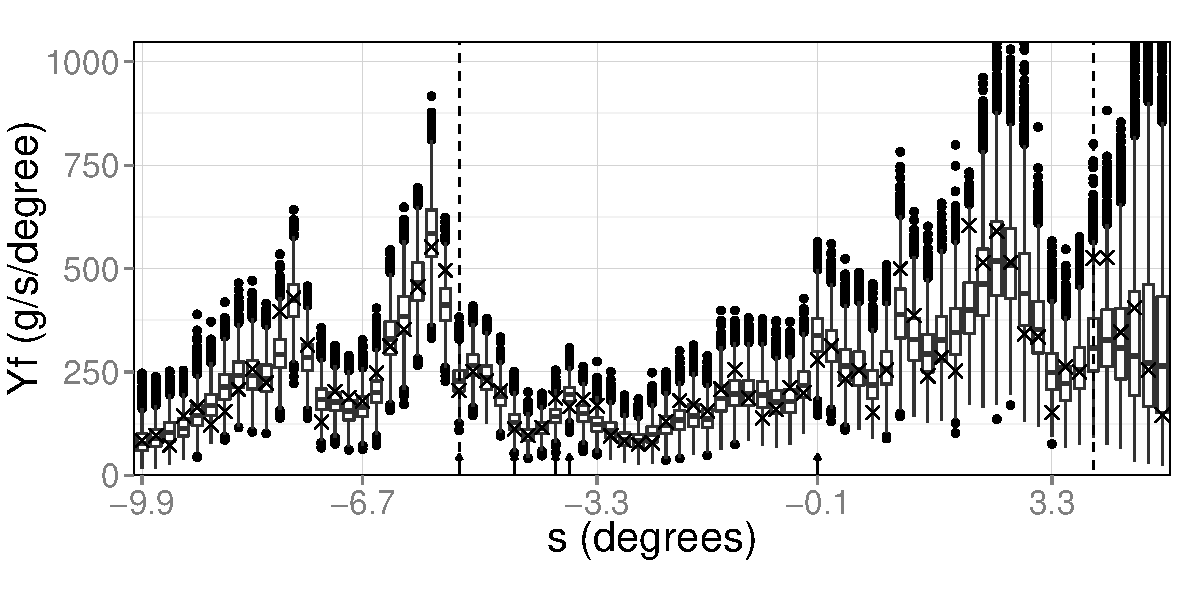
\includegraphics[width=\maxwidth]{figure/HMC-plot-1} 

\end{knitrout}
\end{center}
\caption{Samples from the posterior distribution of the lognormal flux field obtained using Hamiltonian Monte Carlo (HMC). The boxes denote the interquartile range, the whiskers extend to the last values that are within 1.5 times the interquartile range from the quartiles, and the dots show the samples that lie beyond the end of the whiskers. The crosses denote the true (simulated) fluxes, and the arrows denote the locations of the measurements. The vertical dashed lines show the spatial locations analysed in Figure \ref{fig:Lap_vs_mcmc}. Since the observed mole fractions are insensitive to flux at $\{s : s > 4.3\}$, these locations were excluded from the model.}
\label{fig:Slice}
\end{figure}

We now compare the Laplace approximation of the flux field to the distribution given by HMC. We first create a function \texttt{comp\_density} that plots the HMC samples and the Laplace approximation for any arbitrary point, and then pass on two spatial locations to it for plotting:

\begin{knitrout}
\definecolor{shadecolor}{rgb}{0.969, 0.969, 0.969}\color{fgcolor}\begin{kframe}
\begin{alltt}
\hlstd{comp_density} \hlkwb{<-} \hlkwa{function}\hlstd{(}\hlkwc{j}\hlstd{,}\hlkwc{xu}\hlstd{,}\hlkwc{xl}\hlstd{=}\hlnum{0}\hlstd{,}\hlkwc{yu}\hlstd{=}\hlnum{0.01}\hlstd{) \{}
  \hlstd{x} \hlkwb{<-} \hlkwd{seq}\hlstd{(xl,xu,}\hlkwc{by}\hlstd{=}\hlnum{1}\hlstd{)}
  \hlkwd{hist}\hlstd{(q[j,}\hlnum{1}\hlopt{:}\hlstd{(N}\hlopt{-}\hlnum{1}\hlstd{)],}\hlkwc{xlab}\hlstd{=}\hlkwd{c}\hlstd{(}\hlstr{"flux (g/s/degree)"}\hlstd{),}
       \hlkwc{ylab}\hlstd{=}\hlstr{"[Yf | Zm]"}\hlstd{,}
       \hlkwc{main}\hlstd{=}\hlstr{""}\hlstd{,}
       \hlkwc{freq}\hlstd{=F,}
       \hlkwc{xlim}\hlstd{=}\hlkwd{c}\hlstd{(xl,xu),}
       \hlkwc{ylim}\hlstd{=}\hlkwd{c}\hlstd{(}\hlnum{0}\hlstd{,yu))}
  \hlkwd{lines}\hlstd{(x,}\hlkwd{dnorm}\hlstd{(x,}\hlkwc{mean}\hlstd{=X}\hlopt{$}\hlstd{lap_approx}\hlopt{$}\hlstd{Yf[j],}
                \hlkwc{sd}\hlstd{=}\hlkwd{sqrt}\hlstd{(X}\hlopt{$}\hlstd{lap_approx}\hlopt{$}\hlstd{S_ff[j,j])),}
        \hlkwc{lty}\hlstd{=}\hlnum{2}\hlstd{)}
\hlstd{\}}

\hlkwa{if}\hlstd{(}\hlopt{!}\hlstd{misspecification) \{}
  \hlkwd{png}\hlstd{(}\hlstr{"../../density_sim1.png"}\hlstd{,} \hlkwc{width}\hlstd{=}\hlnum{4}\hlstd{,} \hlkwc{height}\hlstd{=}\hlnum{4}\hlstd{,} \hlkwc{units}\hlstd{=}\hlstr{"in"}\hlstd{,} \hlkwc{res}\hlstd{=}\hlnum{300}\hlstd{)}
  \hlkwd{comp_density}\hlstd{(}\hlnum{70}\hlstd{,}\hlnum{800}\hlstd{,}\hlopt{-}\hlnum{200}\hlstd{,}\hlkwc{yu}\hlstd{=}\hlnum{0.005}\hlstd{);} \hlkwd{dev.off}\hlstd{()}
  \hlkwd{png}\hlstd{(}\hlstr{"../../density_sim10.png"}\hlstd{,} \hlkwc{width}\hlstd{=}\hlnum{4}\hlstd{,} \hlkwc{height}\hlstd{=}\hlnum{4}\hlstd{,} \hlkwc{units}\hlstd{=}\hlstr{"in"}\hlstd{,} \hlkwc{res}\hlstd{=}\hlnum{300}\hlstd{)}
  \hlkwd{comp_density}\hlstd{(}\hlnum{24}\hlstd{,}\hlnum{400}\hlstd{,}\hlnum{50}\hlstd{,}\hlkwc{yu}\hlstd{=}\hlnum{0.014}\hlstd{);} \hlkwd{dev.off}\hlstd{()}
\hlstd{\}}
\end{alltt}
\begin{verbatim}
## pdf 
##   2
\end{verbatim}
\end{kframe}
\end{knitrout}


\begin{figure}[!ht]
\begin{center}
\begin{knitrout}
\definecolor{shadecolor}{rgb}{0.969, 0.969, 0.969}\color{fgcolor}\begin{kframe}
\begin{alltt}
\hlkwd{par}\hlstd{(}\hlkwc{mfrow}\hlstd{=}\hlkwd{c}\hlstd{(}\hlnum{1}\hlstd{,}\hlnum{2}\hlstd{))}
\hlkwd{comp_density}\hlstd{(}\hlnum{70}\hlstd{,}\hlnum{800}\hlstd{,}\hlopt{-}\hlnum{200}\hlstd{,}\hlkwc{yu}\hlstd{=}\hlnum{0.005}\hlstd{);}
\hlkwd{comp_density}\hlstd{(}\hlnum{24}\hlstd{,}\hlnum{400}\hlstd{,}\hlnum{50}\hlstd{,}\hlkwc{yu}\hlstd{=}\hlnum{0.014}\hlstd{);}
\end{alltt}
\end{kframe}
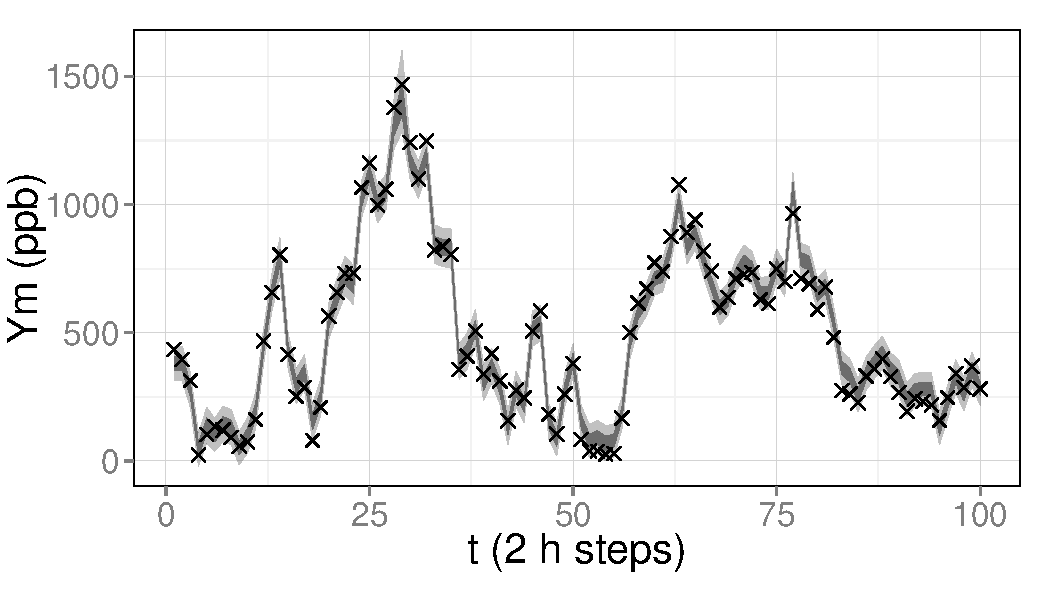
\includegraphics[width=\maxwidth]{figure/unnamed-chunk-8-1} 

\end{knitrout}
\caption{Laplace approximation (dashed line) and a histogram of the empirical posterior distribution from the MCMC samples for the flux at $s = 3.9^\circ$ (left panel) and $s = -5.3^\circ$ (right panel).} \label{fig:Lap_vs_mcmc}
\end{center}
\end{figure}

Having obtained the flux field samples, we now used the collapsing property of the Gibbs sampler to obtain samples for the mole-fraction field by simply running the samples through the forward model:

\begin{knitrout}
\definecolor{shadecolor}{rgb}{0.969, 0.969, 0.969}\color{fgcolor}\begin{kframe}
\begin{alltt}
\hlcom{## Now get the mole fraction samples}
\hlstd{mf_samp} \hlkwb{<-} \hlkwd{matrix}\hlstd{(}\hlnum{0}\hlstd{,}\hlkwd{nrow}\hlstd{(B),N)}                \hlcom{# initialise mole-fraction samples array}
\hlstd{mu_post} \hlkwb{<-} \hlkwd{matrix}\hlstd{(}\hlnum{0}\hlstd{,}\hlkwd{nrow}\hlstd{(B),N)}                \hlcom{# initialise mole-fraction samples array}
\hlstd{Q_post} \hlkwb{<-} \hlkwd{t}\hlstd{(C_m)} \hlopt \hlstd{Qobs} \hlopt \hlstd{C_m} \hlopt{+} \hlstd{Q_zeta}    \hlcom{# conditional precision of Ym}
\hlstd{S_post} \hlkwb{<-} \hlkwd{chol2inv}\hlstd{(}\hlkwd{chol}\hlstd{(Q_post))}              \hlcom{# conditional covariance of Ym}
\hlstd{L_S_post} \hlkwb{<-} \hlkwd{t}\hlstd{(}\hlkwd{chol}\hlstd{(S_post))}                   \hlcom{# Cholesky decomposition of above}
\hlstd{SQB} \hlkwb{<-} \hlstd{S_post} \hlopt \hlstd{Q_zeta} \hlopt \hlstd{B[,X}\hlopt{$}\hlstd{ind]}        \hlcom{# weight given to flux sample}
\hlstd{StCQoz} \hlkwb{<-} \hlstd{S_post} \hlopt \hlkwd{t}\hlstd{(C_m)} \hlopt \hlstd{Qobs} \hlopt \hlstd{s_obs}\hlopt{$}\hlstd{z} \hlcom{# influence of observation}
\hlkwa{for} \hlstd{(i} \hlkwa{in} \hlnum{1}\hlopt{:}\hlstd{N)\{}
 \hlstd{mu_post[,i]} \hlkwb{<-} \hlkwd{as.vector}\hlstd{(SQB} \hlopt \hlstd{q[,i]} \hlopt{+}     \hlcom{# conditional mean}
                            \hlstd{StCQoz)}
 \hlstd{mf_samp[,i]} \hlkwb{<-} \hlkwd{as.vector}\hlstd{(mu_post[,i]} \hlopt{+}       \hlcom{# generate sample}
                            \hlstd{L_S_post} \hlopt \hlkwd{rnorm}\hlstd{(}\hlkwd{nrow}\hlstd{(B)))}
\hlstd{\}}
\end{alltt}
\end{kframe}
\end{knitrout}

Now that we have our mole-fraction samples we can plot the credibility intervals at the unobserved location. We do this by taking the 6th row (recall that $m = 6$) of the mole-fraction samples matrix, putting the rows into a data frame and plotting the result.
\begin{knitrout}
\definecolor{shadecolor}{rgb}{0.969, 0.969, 0.969}\color{fgcolor}\begin{kframe}
\begin{alltt}
\hlstd{stat1} \hlkwb{<-}  \hlkwd{seq}\hlstd{(}\hlnum{6}\hlstd{,}\hlnum{600}\hlstd{,}\hlkwc{by}\hlstd{=}\hlnum{6}\hlstd{)}
\hlstd{mu} \hlkwb{<-} \hlkwd{apply}\hlstd{(mf_samp[stat1,}\hlopt{-}\hlkwd{c}\hlstd{(}\hlnum{1}\hlopt{:}\hlnum{1000}\hlstd{,i)],}\hlnum{1}\hlstd{,median)}
\hlstd{uq} \hlkwb{<-} \hlkwd{apply}\hlstd{(mf_samp[stat1,}\hlopt{-}\hlkwd{c}\hlstd{(}\hlnum{1}\hlopt{:}\hlnum{1000}\hlstd{,i)],}\hlnum{1}\hlstd{,quantile,}\hlnum{0.75}\hlstd{)}
\hlstd{lq} \hlkwb{<-} \hlkwd{apply}\hlstd{(mf_samp[stat1,}\hlopt{-}\hlkwd{c}\hlstd{(}\hlnum{1}\hlopt{:}\hlnum{1000}\hlstd{,i)],}\hlnum{1}\hlstd{,quantile,}\hlnum{0.25}\hlstd{)}
\hlstd{uuq} \hlkwb{<-} \hlkwd{apply}\hlstd{(mf_samp[stat1,}\hlopt{-}\hlkwd{c}\hlstd{(}\hlnum{1}\hlopt{:}\hlnum{1000}\hlstd{,i)],}\hlnum{1}\hlstd{,quantile,}\hlnum{0.95}\hlstd{)}
\hlstd{llq} \hlkwb{<-} \hlkwd{apply}\hlstd{(mf_samp[stat1,}\hlopt{-}\hlkwd{c}\hlstd{(}\hlnum{1}\hlopt{:}\hlnum{1000}\hlstd{,i)],}\hlnum{1}\hlstd{,quantile,}\hlnum{0.05}\hlstd{)}
\hlstd{df} \hlkwb{<-} \hlkwd{data.frame}\hlstd{(}\hlkwc{mean} \hlstd{= mu,} \hlkwc{uq}\hlstd{=uq,}\hlkwc{lq}\hlstd{=lq,}\hlkwc{uuq}\hlstd{=uuq,}\hlkwc{llq}\hlstd{=llq,}\hlkwc{t}\hlstd{=}\hlnum{1}\hlopt{:}\hlkwd{length}\hlstd{(mu))}

\hlstd{g} \hlkwb{<-} \hlkwd{LinePlotTheme}\hlstd{()} \hlopt{+}
  \hlkwd{geom_ribbon}\hlstd{(}\hlkwc{data}\hlstd{=df,}\hlkwd{aes}\hlstd{(}\hlkwc{x}\hlstd{=t,}\hlkwc{ymax}\hlstd{=uq,}\hlkwc{ymin}\hlstd{=lq),}\hlkwc{alpha}\hlstd{=}\hlnum{0.6}\hlstd{)} \hlopt{+}
  \hlkwd{geom_ribbon}\hlstd{(}\hlkwc{data}\hlstd{=df,}\hlkwd{aes}\hlstd{(}\hlkwc{x}\hlstd{=t,}\hlkwc{ymax}\hlstd{=uuq,}\hlkwc{ymin}\hlstd{=llq),}\hlkwc{alpha}\hlstd{=}\hlnum{0.3}\hlstd{)} \hlopt{+}
  \hlkwd{geom_point}\hlstd{(}\hlkwc{data}\hlstd{=}\hlkwd{subset}\hlstd{(s_obs_old,s}\hlopt{==}\hlstd{new_obs),}
             \hlkwd{aes}\hlstd{(}\hlkwc{x}\hlstd{=t,}\hlkwc{y} \hlstd{= z),}\hlkwc{colour}\hlstd{=}\hlstr{'black'}\hlstd{,}\hlkwc{size}\hlstd{=}\hlnum{3}\hlstd{,}\hlkwc{shape}\hlstd{=}\hlnum{4}\hlstd{)}\hlopt{+}
    \hlkwd{ylab}\hlstd{(}\hlstr{"Ym (ppb)"}\hlstd{)} \hlopt{+} \hlkwd{xlab}\hlstd{(}\hlstr{"t (2 h steps)"}\hlstd{)}

\hlkwa{if}\hlstd{(}\hlopt{!}\hlstd{misspecification)}
  \hlkwd{ggsave}\hlstd{(}\hlstr{"../../MF_samples.png"}\hlstd{,}\hlkwc{plot} \hlstd{= g,}\hlkwc{width}\hlstd{=}\hlnum{10}\hlstd{,}\hlkwc{height}\hlstd{=}\hlnum{3}\hlstd{)}
\end{alltt}
\end{kframe}
\end{knitrout}

\begin{figure}[!ht]
\begin{center}
\begin{knitrout}
\definecolor{shadecolor}{rgb}{0.969, 0.969, 0.969}\color{fgcolor}\begin{kframe}
\begin{alltt}
\hlkwd{print}\hlstd{(g)}
\end{alltt}
\end{kframe}
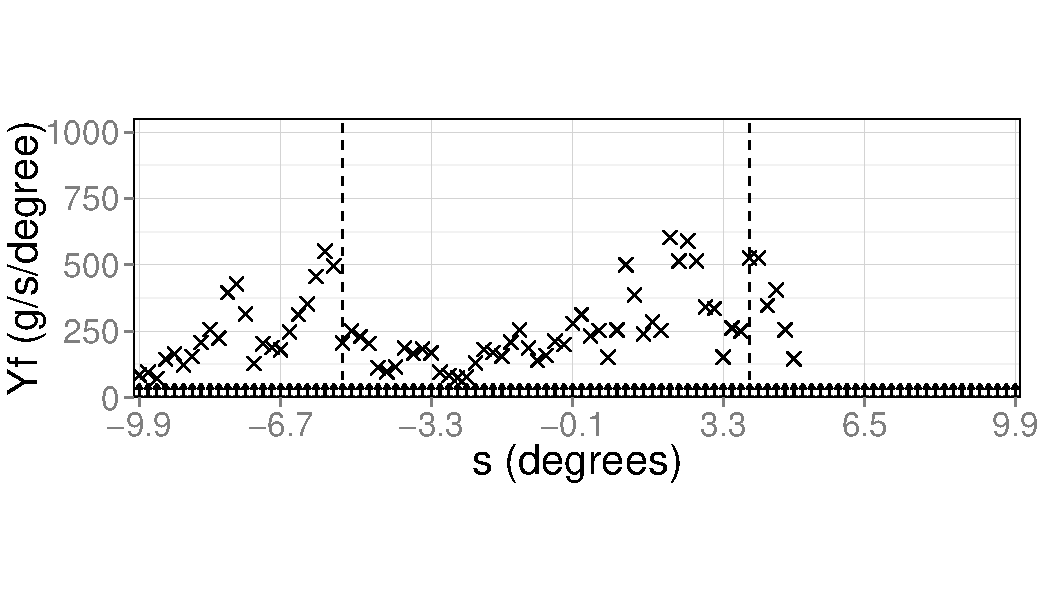
\includegraphics[width=\maxwidth]{figure/unnamed-chunk-9-1} 

\end{knitrout}
\caption{Distributions of mole fraction at $s = 0.3^\circ$ and $t \in \mathcal{T}$, following Gibbs sampling. The dark and light shadings denote the interquartile and the 5--95 percentile ranges, respectively. The crosses denote the true (simulated) mole fractions.} \label{fig:MF}
\end{center}
\end{figure}

Finally, we calculate the statistics $S_{1,f}$, $S_{2,f}$ and $S_{1,m}^{0.3}$ as defined in the paper:

\begin{knitrout}
\definecolor{shadecolor}{rgb}{0.969, 0.969, 0.969}\color{fgcolor}\begin{kframe}
\begin{alltt}
\hlcom{# Flux errors}
\hlstd{residual} \hlkwb{<-}\hlstd{(st_grid}\hlopt{$}\hlstd{Yf[}\hlnum{1}\hlopt{:}\hlnum{75}\hlstd{]} \hlopt{-} \hlkwd{apply}\hlstd{(q,}\hlnum{1}\hlstd{,mean))}
\hlstd{post_unc} \hlkwb{<-} \hlkwd{apply}\hlstd{(q,}\hlnum{1}\hlstd{,var)}
\hlkwd{print}\hlstd{(}\hlkwd{paste0}\hlstd{(}\hlstr{"S1f = "}\hlstd{,} \hlkwd{sqrt}\hlstd{(}\hlkwd{mean}\hlstd{(residual}\hlopt{^}\hlnum{2}\hlstd{))))}
\end{alltt}
\begin{verbatim}
## [1] "S1f = 286.704308542919"
\end{verbatim}
\begin{alltt}
\hlkwd{print}\hlstd{(}\hlkwd{paste0}\hlstd{(}\hlstr{"S2f = "}\hlstd{,} \hlkwd{sqrt}\hlstd{(}\hlkwd{mean}\hlstd{(residual}\hlopt{^}\hlnum{2}\hlstd{)} \hlopt{/}\hlkwd{mean}\hlstd{(post_unc))))}
\end{alltt}
\begin{verbatim}
## [1] "S2f = Inf"
\end{verbatim}
\begin{alltt}
\hlcom{# MF errors}
\hlstd{residual} \hlkwb{<-} \hlstd{(}\hlkwd{apply}\hlstd{(mf_samp[rm_idx,],}\hlnum{1}\hlstd{,mean)} \hlopt{-} \hlkwd{subset}\hlstd{(st_grid,s} \hlopt{==} \hlstd{new_obs)}\hlopt{$}\hlstd{Ym)}
\hlstd{post_unc} \hlkwb{<-} \hlkwd{apply}\hlstd{(mf_samp[rm_idx,],}\hlnum{1}\hlstd{,var)}
\hlkwd{print}\hlstd{(}\hlkwd{paste0}\hlstd{(}\hlstr{"S1m = "}\hlstd{,} \hlkwd{sqrt}\hlstd{(}\hlkwd{mean}\hlstd{(residual}\hlopt{^}\hlnum{2}\hlstd{))))}
\end{alltt}
\begin{verbatim}
## [1] "S1m = 269.296985979694"
\end{verbatim}
\end{kframe}
\end{knitrout}


\end{document}
